%%-----------------Chapter 6---------------------------
% \documentclass[../UNBThesis2.tex]{subfiles}
\setlength{\parindent}{2em}
%%%%%%%%%% NUMber of centrers + run time -memory.....
%%%%%%%% winodow length+ all validation metrics




% %\colorbox{yellow}{one week --AP/ Kmeans(same week)--> first week int }
% % \colorbox{yellow}{one day position/count(same day)} %Friday, October 30, 3987 --monday(first day of inter)i
% % \colorbox{yellow}{update hourly one day(same day -5/1)} --> one day AP 
% \colorbox{yellow}{summary plot -->waterfall evolution - one week po cou tim } cluster center???
% \colorbox{yellow}{LBAP -one week }
% % \colorbox{yellow}{DSAP one week}
% \colorbox{yellow}{streaming Kmeans --one week???}

% \colorbox{yellow}{DSAP 3 seprate month}
% \colorbox{yellow}{Streaming Kmeans 3 sep month}
% % \colorbox{yellow}{one month Kmeans}
% \colorbox{yellow}{waterfal one month --> x: month y: position z: number of people }

% \begin{document}
\chapter{Discussion of the Results}

%\subsubsection{Comparison between DSAP and streaming K-means Phase}: The aim is to demonstrate the relevance of the proposed DSAP approach compared to streaming K-means algorithm. very important to explain why streaming kemans: - difficult to find available source code from previusouly proposed stream AP, etc...online)no offline) - no window
% \section{Validation of DSAP Algorithm}
% \section{Experimentation on Dataset}
% \section{experimental results}
% \section{Experiments with real-world e-counter data}

time interval used is one hour for ecounters
time interval used was 10 minutes for wifi



to show the results:

Ecounters 

descriptive: entire experiment/distribution: Fig 6.1. daily total number of counts for the entire experiment time. White: two weeks off for the March break, 6.2 gree in friday, orange is tuesday, fig 6.3, fig 6.4,  fig 6.5 (we need the other two blocks), maybe 6.6 is not needed(Nasrin, if you find an interpretation that is relevant)>>>>> we have all these figures, but the conclusion is that the campaign has not worked, not motivated people to take the stairs... time of the experiment was the end of the semester...

AP (weekly patterns)

fig. 8: Comparison of cluster patterns found during one week of before, during, and after intervention
clusters for one week of data ( data points, and numbers show how many data points a cluster has, colour represents the clusters) before the intervention 
one week of data before intervention
you will add
one week of data during the intervention
one week of data after the intervention

Kmeans >>>  OUT
fig 6.9: same week as before, same data as fig 8, but running kmeans


DSAP
CLUSTER EVOLUTION
fig.7: show the hourly evolution of the micro-cluster for each time window for one day during intervention.
fig 20: will show the monthly evolution through the beginning, during, and after the experiment. 

EVALUATION (PERFORMANCE, QUALITY)
New Figure
one week of data before the intervention
one week of data during the intervention
one week of data after the intervention
same weeks that you have used in AP Fig 8
to show how many micro-clusters belong to a macro-cluster
if it is too complicated, make a table.
PURPOSE: With AP and DSAP: we found the same patterns or not???

Combine the three tables:highlight the table with the results that we are going to discuss in detail
Table 6.1 : one week before the intervention
Table 6.2  : one week during
Table 6.3 : one week after
the same weeks that have been used for the figures
PURPOSE: to know if get similar performance and quality results for the 3 weeks. = to prove that DSAP is robust








In this chapter, data from the e-counter and WiFi Indoor Localization experiments are analyzed using the AP, K-means, and the DSAP clustering algorithms to gain insights into the measurements. We demonstrate the strengths and weaknesses of AP and discuss how DSAP provides potential solutions to these. Data stream clustering results are also compared with the results from the streaming K-means algorithm. 

Both the experiments provide information regarding occupant's behaviour and movement within a confined space. The details of the experiments and the analysis tools have already been discussed in the last two Chapters. In the following sections, the data sets will be explained in detail, and the patterns identified by the clustering methods will be analyzed.

 
\section{Behavioural Intervention Experiment} 


\begin{figure}[!h]
    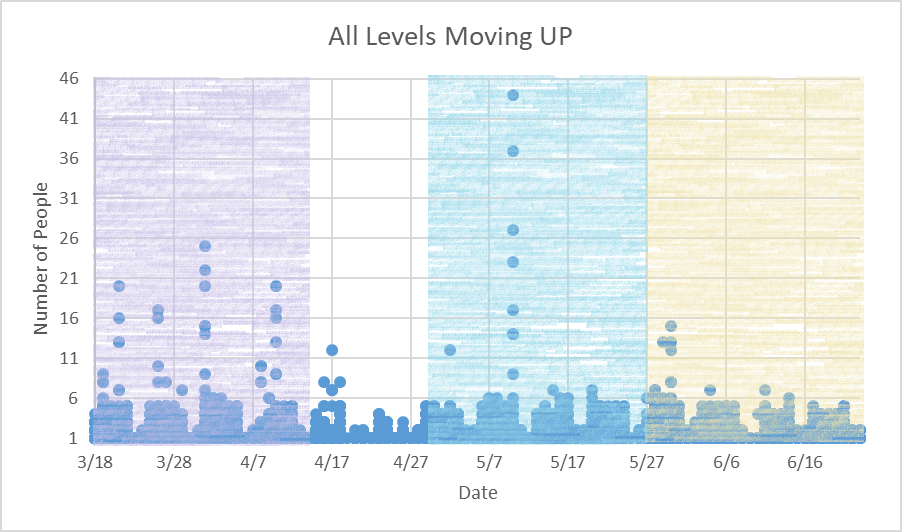
\includegraphics[width=\textwidth]{image/up.png}\hfill
    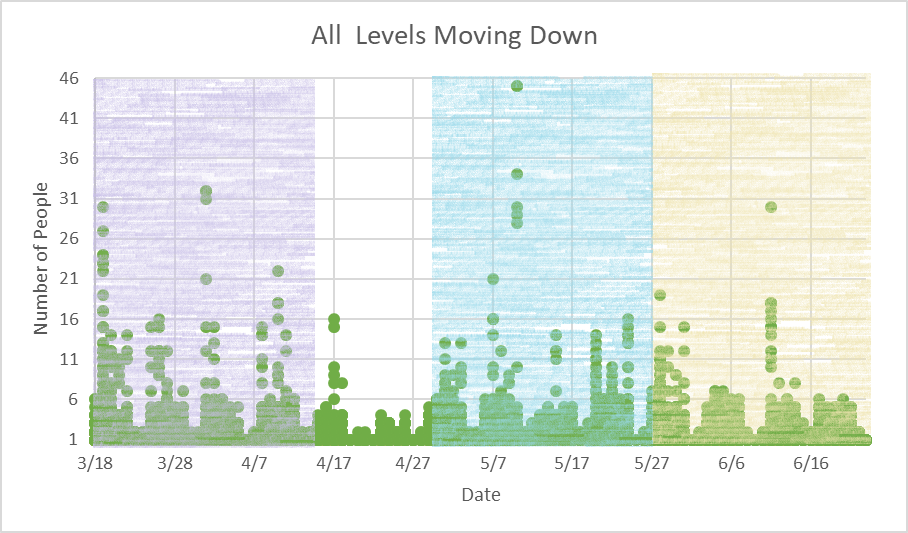
\includegraphics[width=\textwidth]{image/down.png}
    % \\[\smallskipamount]
    \caption{The total number of people using the stairs for the entire period. The purple, blue and yellow highlighted regions show the baseline, intervention, and follow up periods.}
    \label{updown}
\end{figure}

The people counter sensors located at the stairs of the Tonsley building log several parameters. The most relevant parameters for the current study are the location of the sensors and the number of people passing through the sensors. These accurate integer-valued parameters not only indicate the number of people occupying any particular floor but also accurately determine the number of people using the stairs in any particular direction.

The entire data set split by the direction of stair use is shown in Figure \ref{updown}. The three periods of control, intervention, and post-intervention are highlighted with purple, blue, and yellow shaded regions. It is quite apparent that people prefer taking the stairs to go down rather than up. An expected periodic lower occupancy is also observed on the weekends. The mid-semester break from April 15-28 was excluded from the study as that represented anomalous behavior.

To gain further insights in to the data, the total number of people using the stairs (both up and down) over each month of the experiment are plotted in Figure \ref{3mon} to show daily variations in the stairs usage. No visible patterns in the daily variation of stair usage are observed.  Although a noticeable pattern in the hourly movement is consistently seen. The peak stair usage is around noon most probably during the lunch break. The people count is asymmetric on both sides of the peak, with more people using the stairs in the afternoon. But the presence of a higher number of people in the afternoon biasing the results can not be discounted. % these observations can also be made from the next figure.


% It can be clearly seen that the people's activity is the highest at the start of the week on Monday and Tuesday. The sensor count drops from Wednesday to Friday but has similar characteristics while the weekends as expected are very quiet. % Only applicable for a week of observation 



 
\begin{figure}[htbp]
    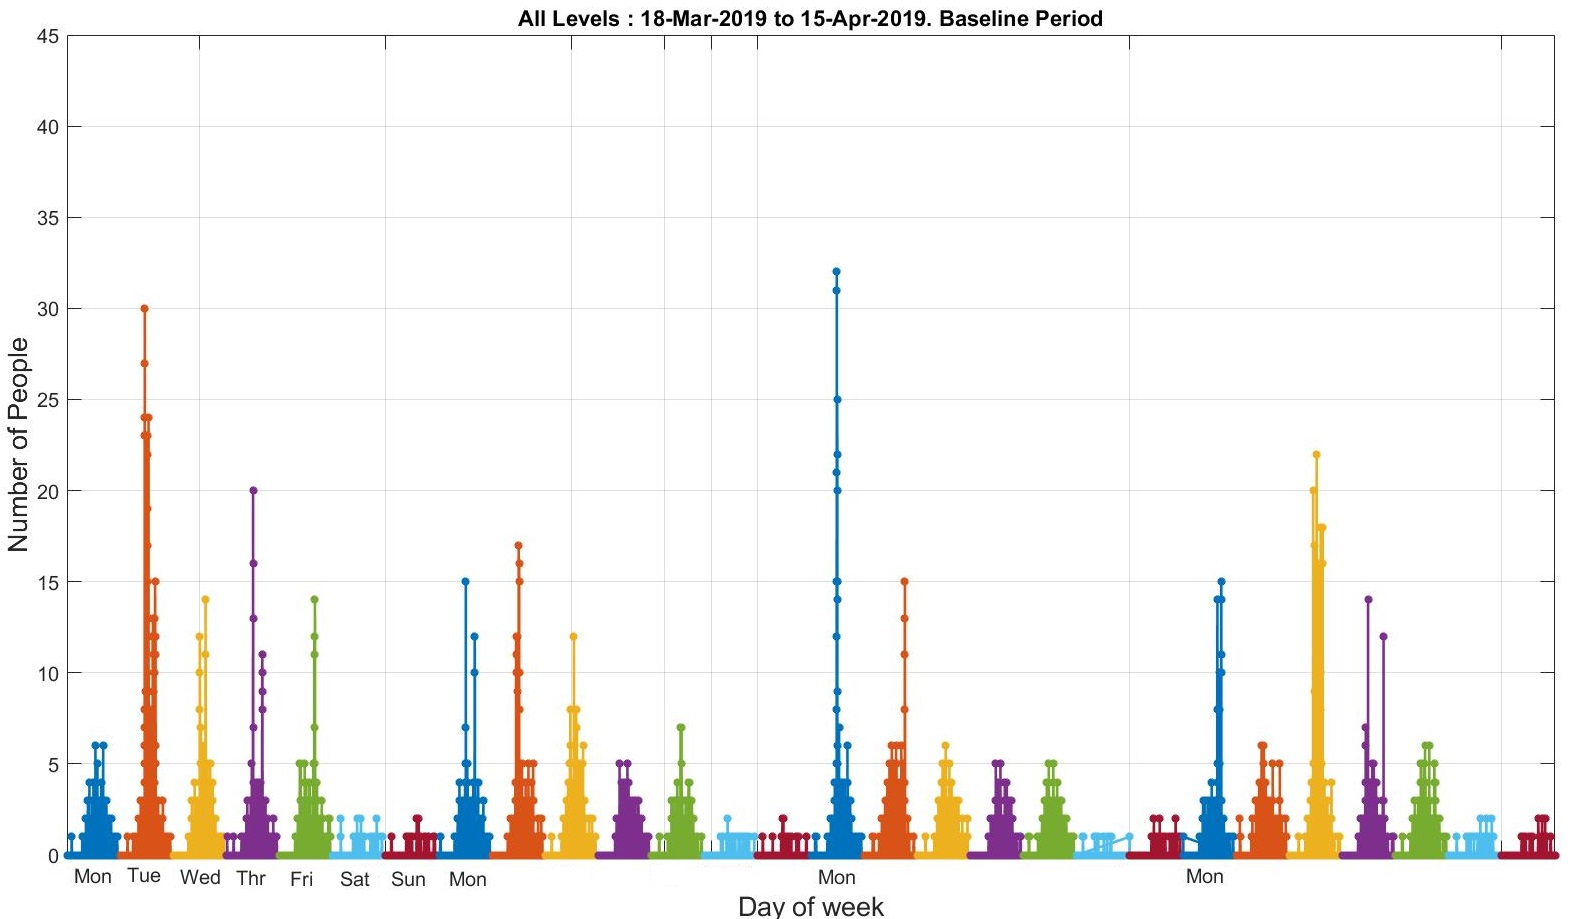
\includegraphics[width=0.8\textwidth]{image/Chapters/Chapter6/18-Mar-2019Base.jpg}
    % \hfill
    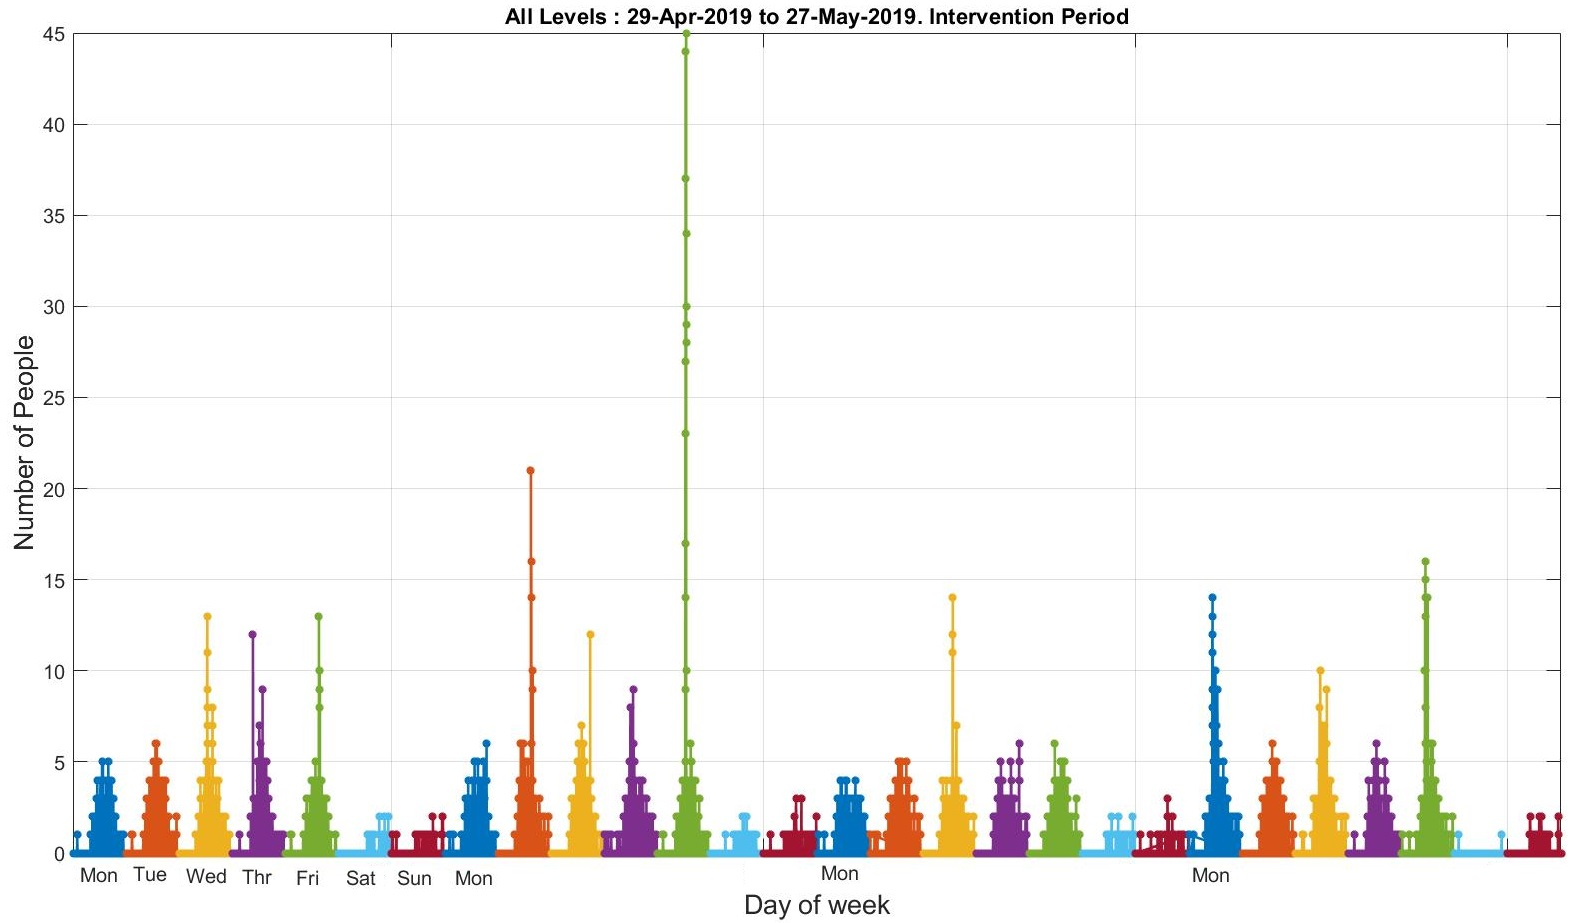
\includegraphics[width=0.8\textwidth]{image/Chapters/Chapter6/29-Apr-2019Int.jpg}
    % \hfill
    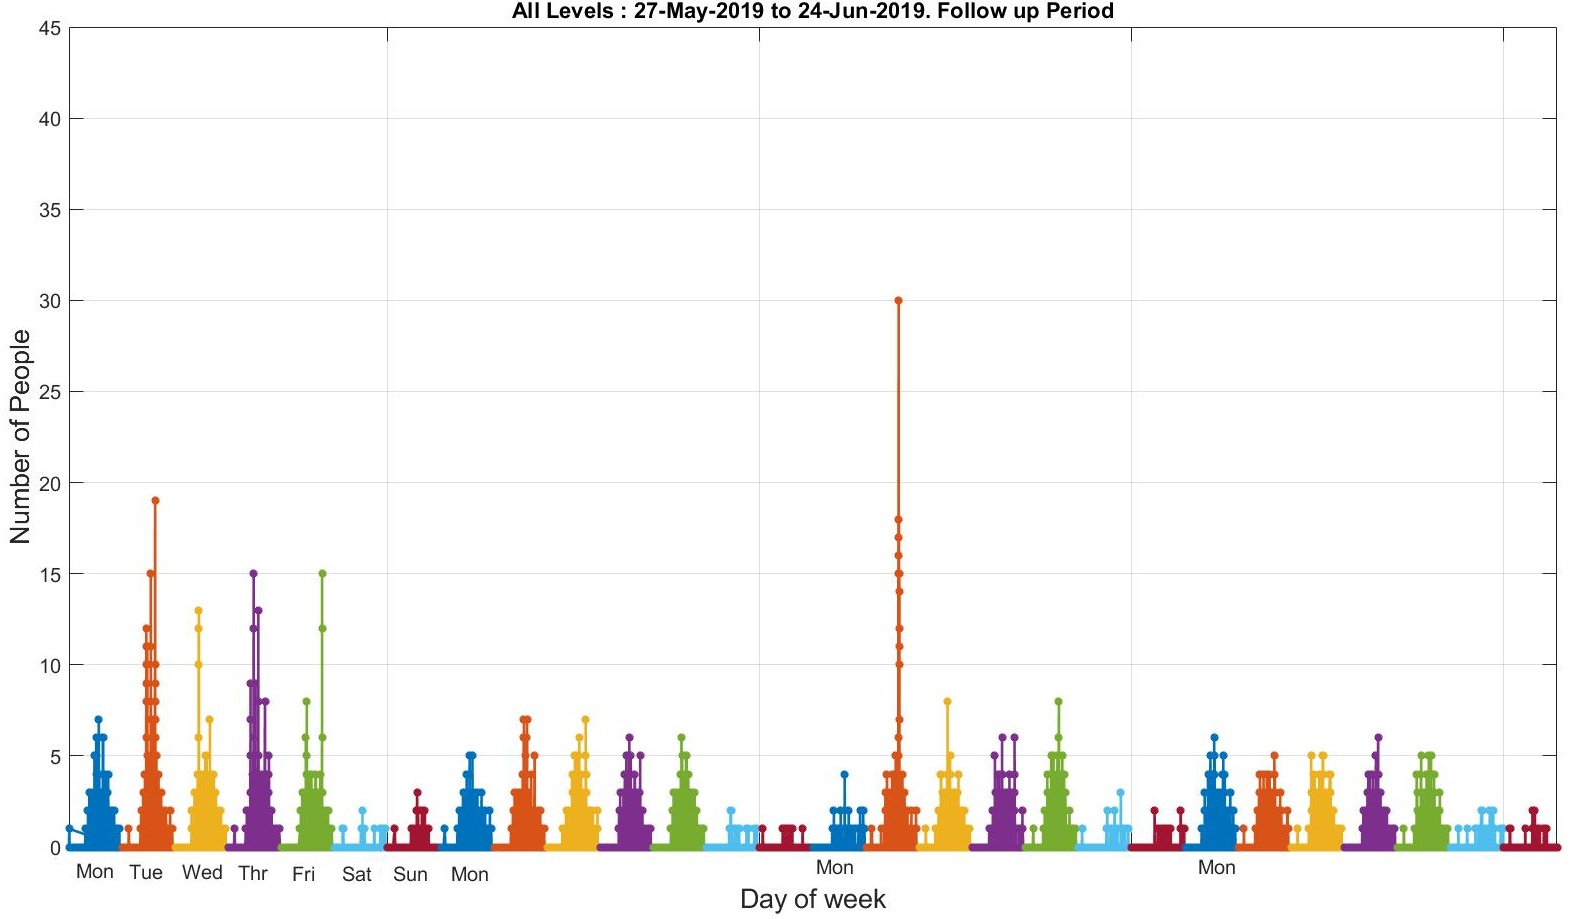
\includegraphics[width=0.8\textwidth]{image/Chapters/Chapter6/27-May-2019Follow.jpg}
    % \\[\smallskipamount]
    \caption{The total number of people using the stairs before, after and during intervention.}
    % \caption{The total number of people using the stairs during the pre-intervention month}
    \label{3mon}
\end{figure}

The Spatio-temporal distribution of stair-usage at each level as shown in Figure \ref{spa1} was generated by aggregating the number of people at each level for each of the months under observation. It is clear that Level 2-1 stair are the most used by people while levels 4-3 North and 5-4 North are used the least. This could be due to fewer people using the north entrances (look at Figure \ref{tons} for reference). These aggregated plots too confirm that the daily peak in activity is around noon. The asymmetry in people count on both sides of the peak is seen in these plots as well. This signifies that consistently more number of people use the stairs in the afternoon as compared to the morning. Although the overall trend of the number of people at each level remains consistent for the three months but an increase at each level is observed during the month of intervention which warrants further study.

\begin{figure}[tpb]
    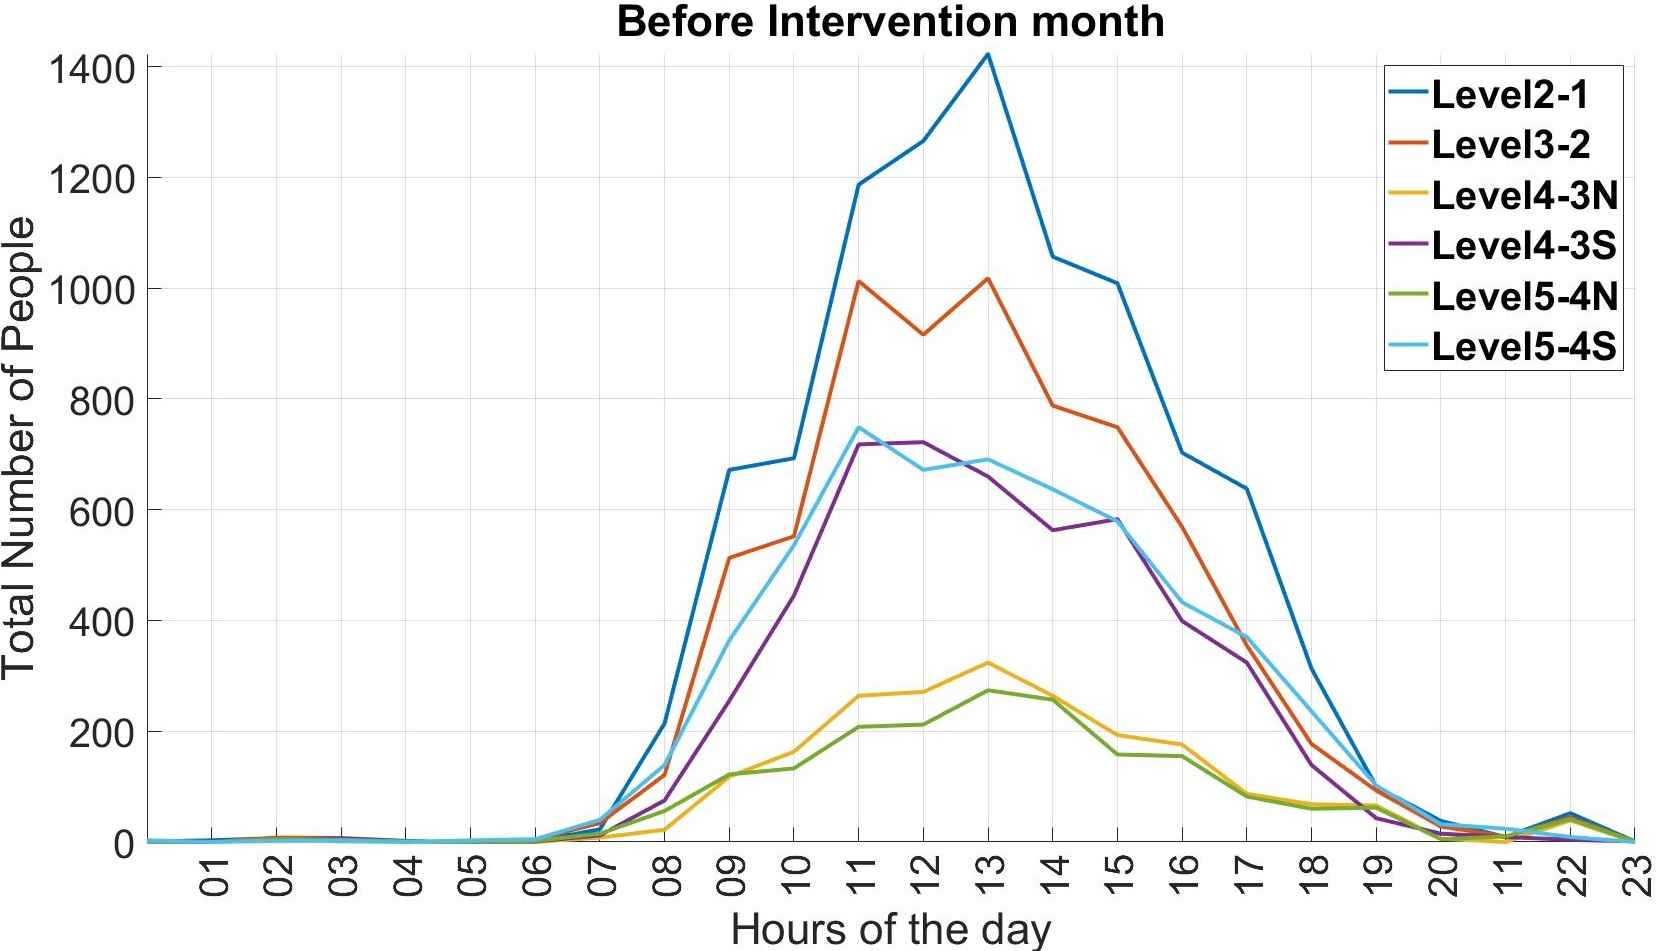
\includegraphics[width=.5\textwidth]{image/before_int.jpg}\hfill
    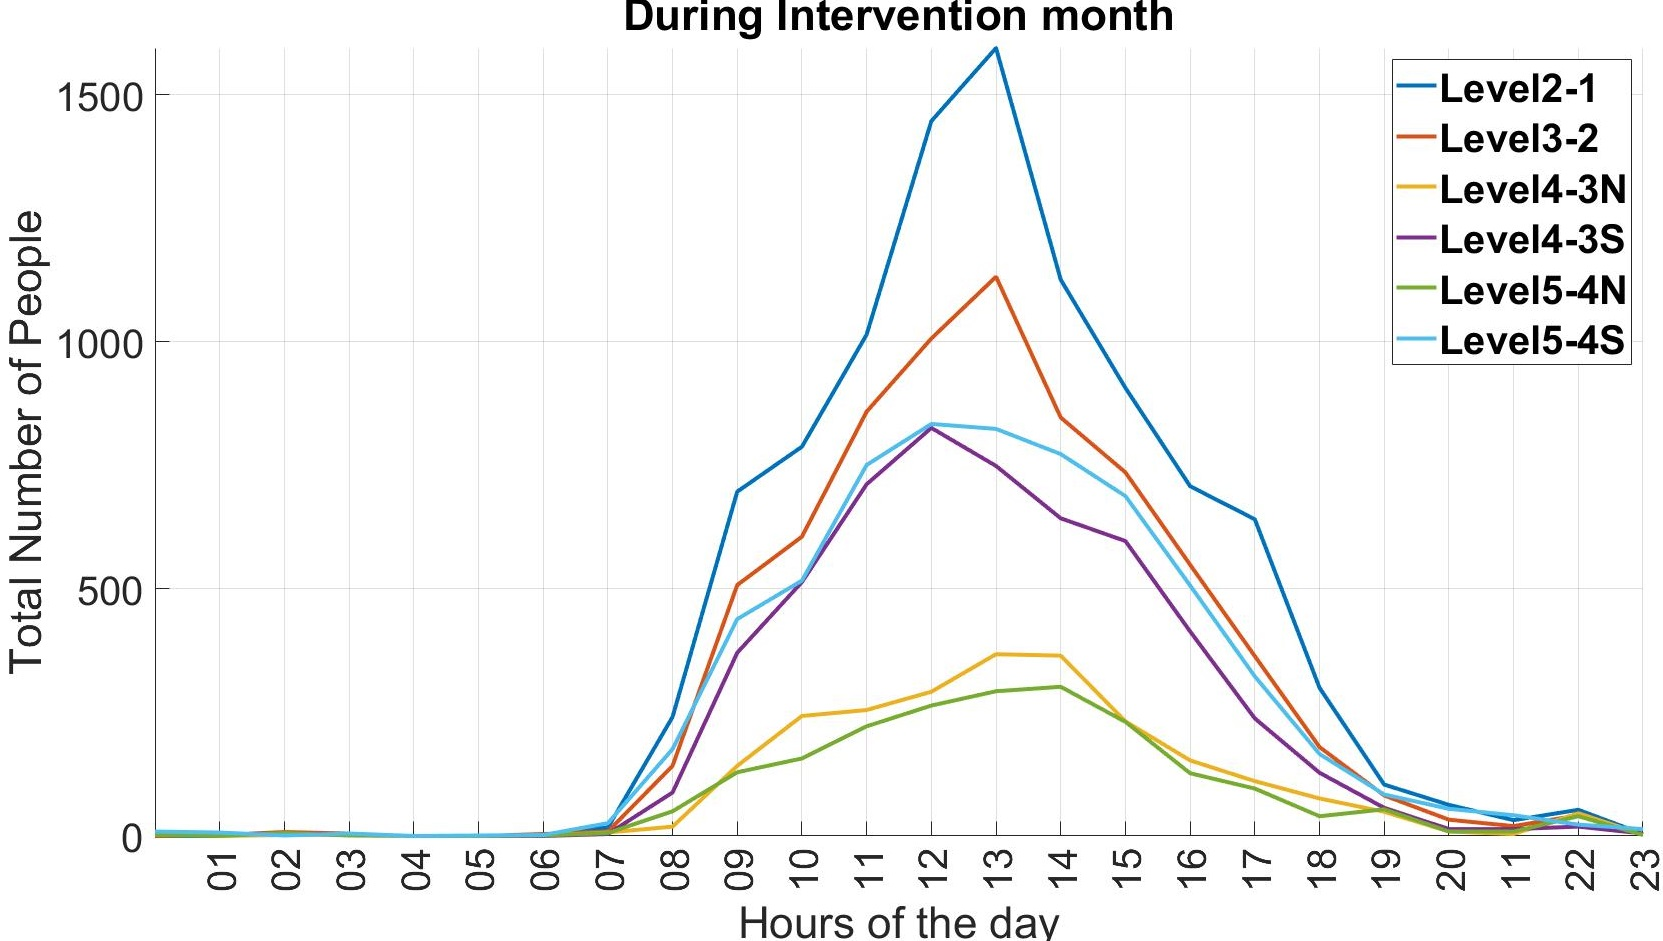
\includegraphics[width=.5\textwidth]{image/during_int.jpg}\hfill\centering
    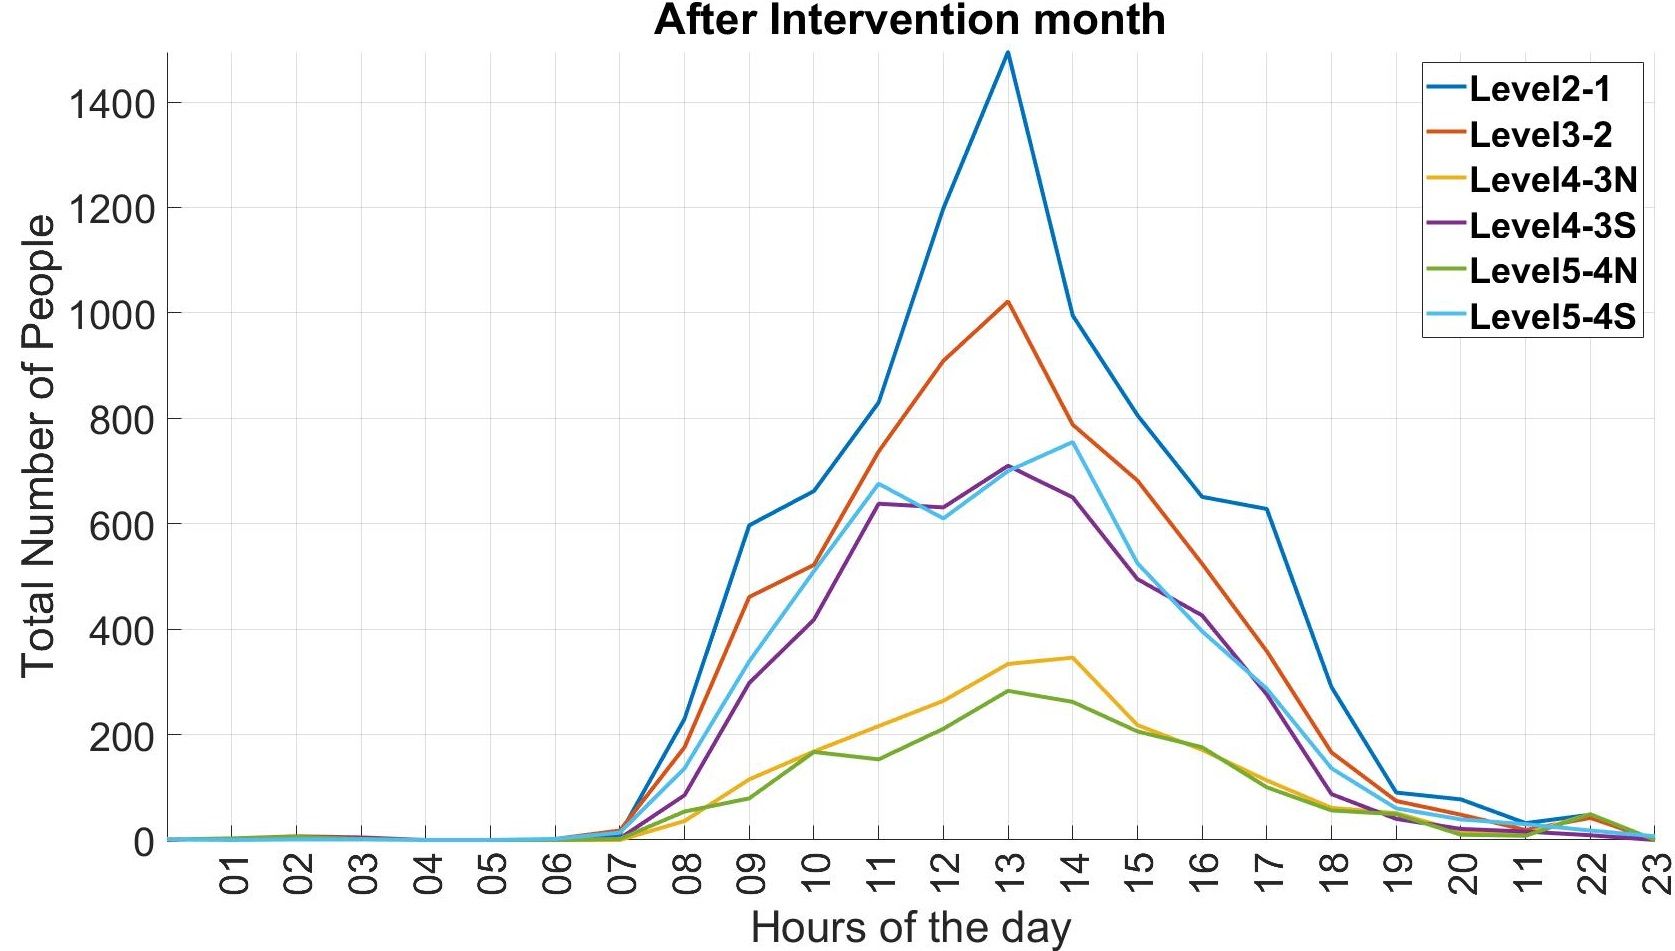
\includegraphics[width=.5\textwidth]{image/after_int.jpg}
    \\[\smallskipamount]
    \caption{Spatio-temporal distribution of the aggregated stair usage during the period of intervention.}
    \label{spa1}
\end{figure}

The aggregated weekly distribution of stair usage for the three periods is plotted in Figure \ref{spa2}. No discernible differences in the distribution are observed between each day of the week for all three months. However, just like the Spatio-temporal representation in the Figure. \ref{spa1} here, too a general increase on all days is observed during the intervention month. The typical daily usage pattern can be grouped into four zones as shown in Figure \ref{timegrup}. The peak activity is clearly around noon and 1 p.m., which show similar patterns. The pre-noon and post-noon activities at 11 a.m., 2 p.m., and 3 p.m. are the periods with the next highest activity. Most of the measurements were made during the late evening and early morning hours when the number of people inside the building was unexpectedly low. The last group consists of the hours with moderate activity seen at the start and end of the workday. 



\begin{figure}[htbp]
    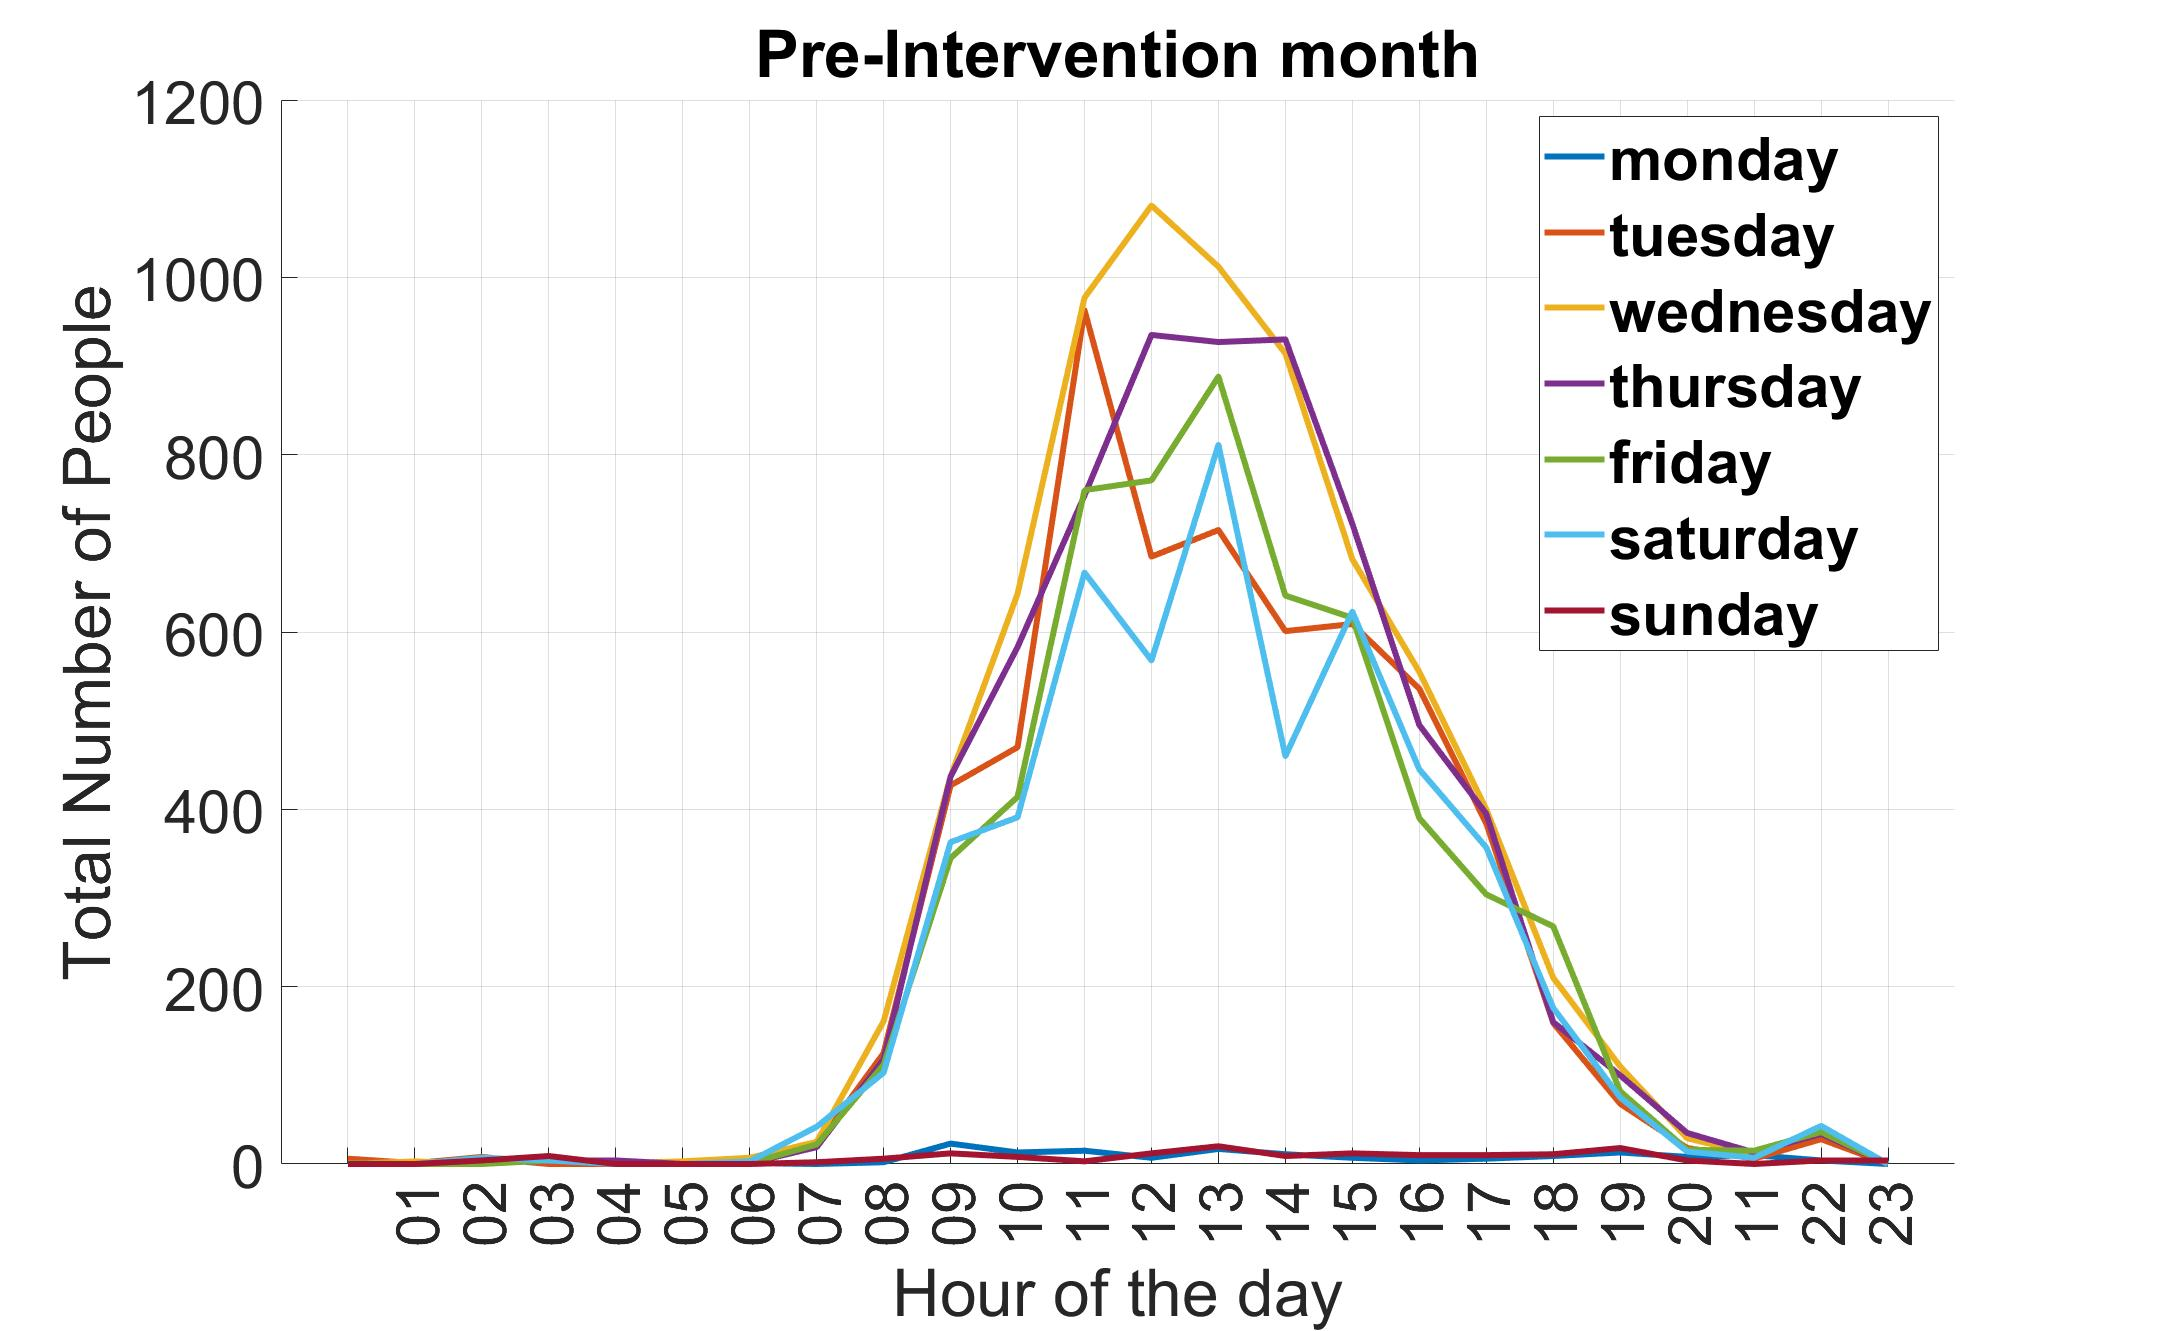
\includegraphics[width=.5\textwidth]{image/aggWeekPre.jpg}\hfill
    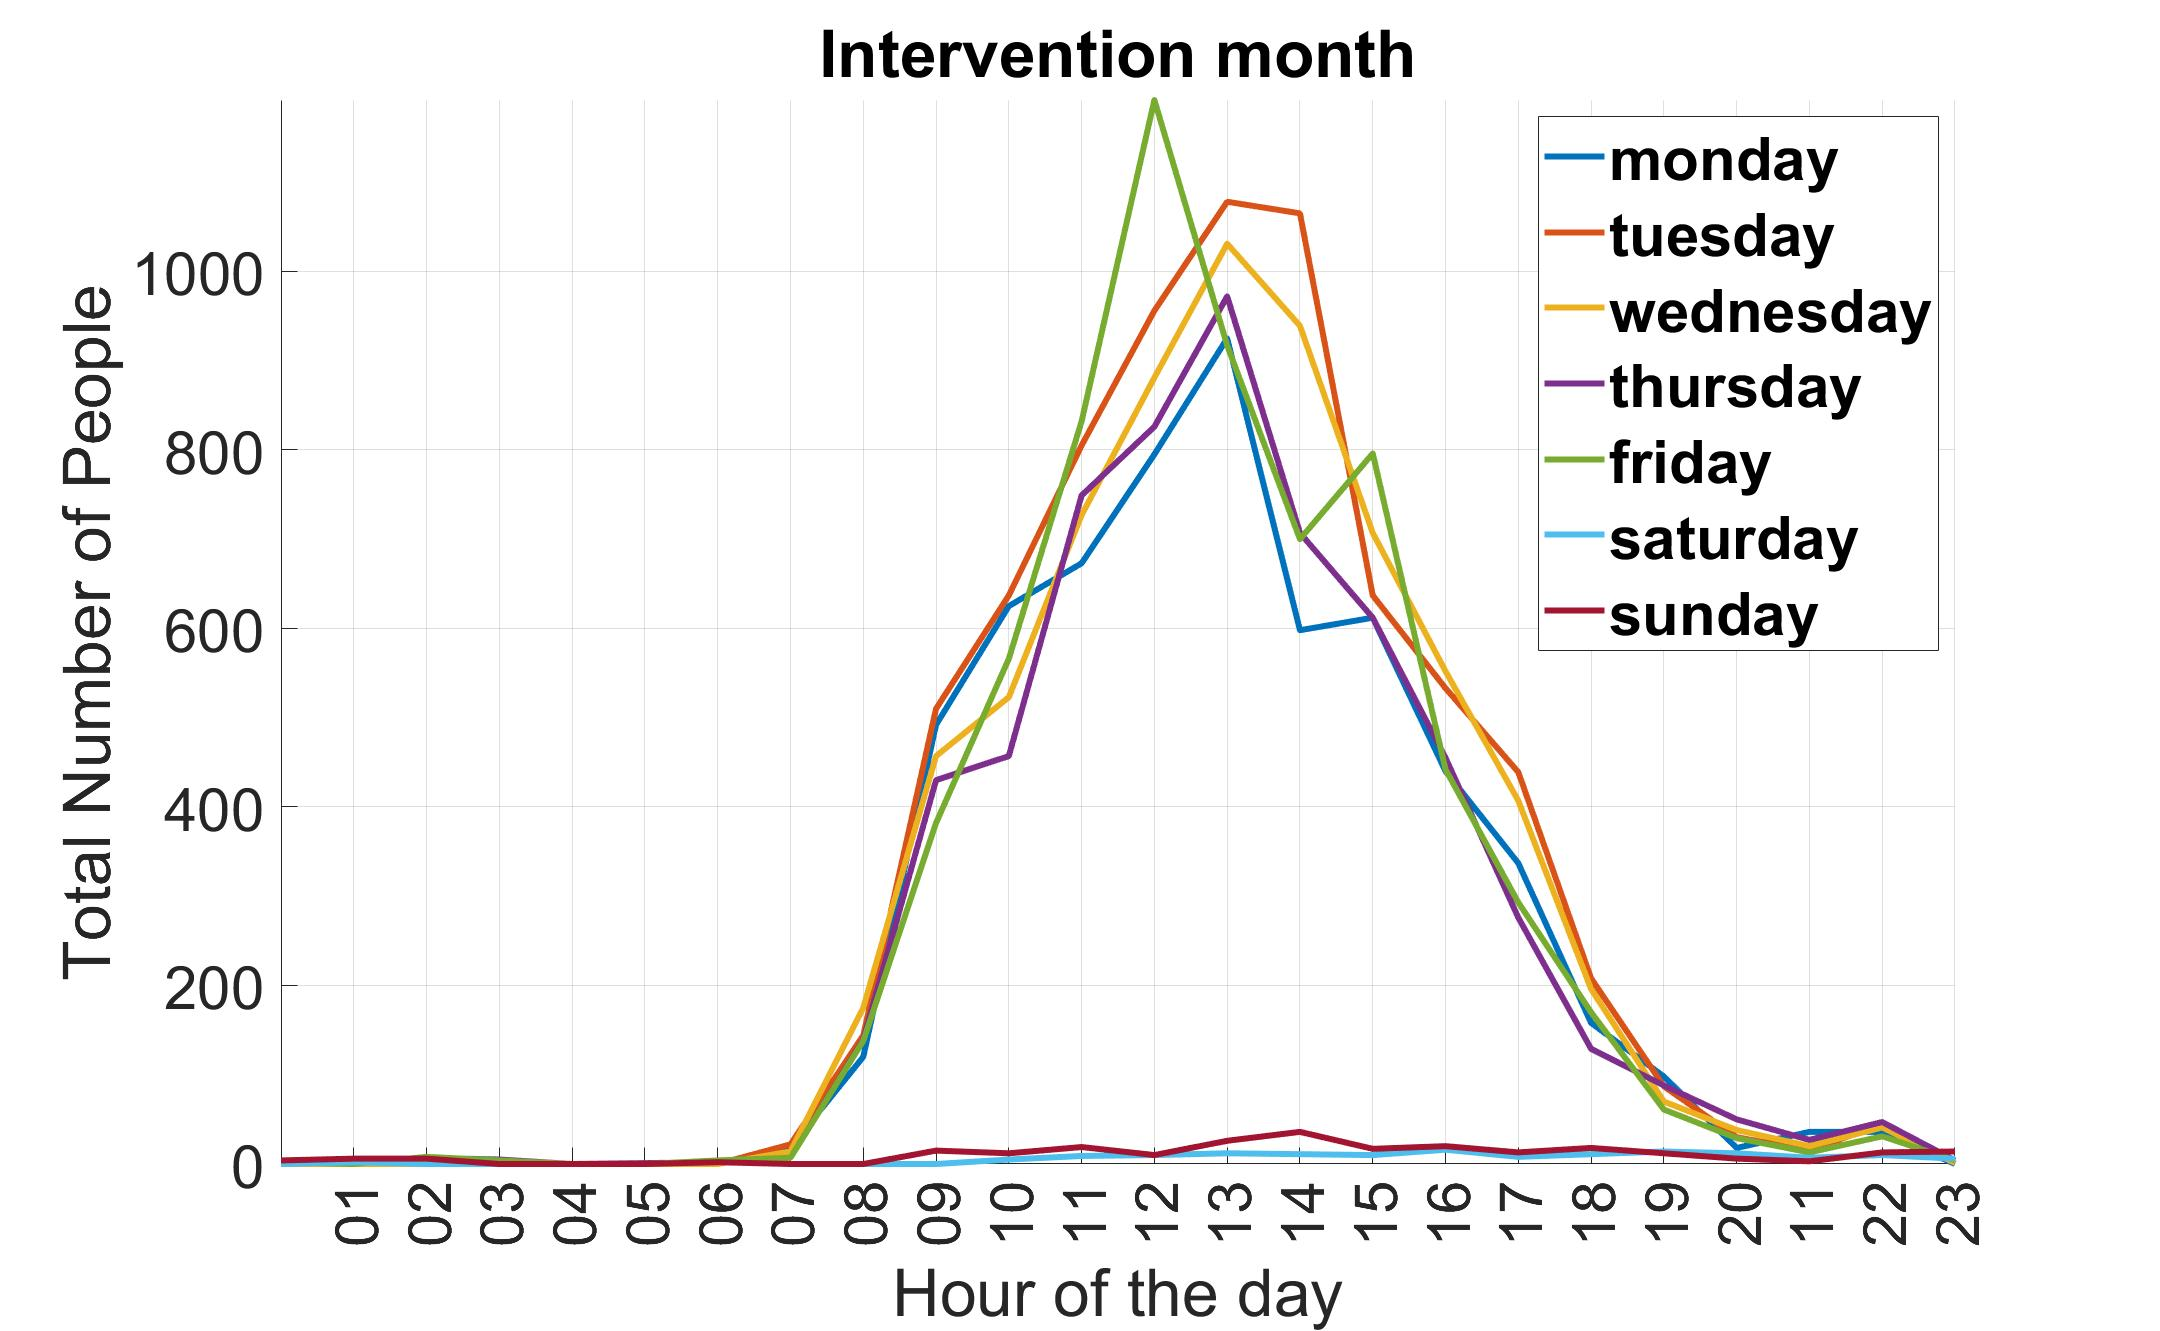
\includegraphics[width=.5\textwidth]{image/aggWeekInt.jpg}\hfill\centering
    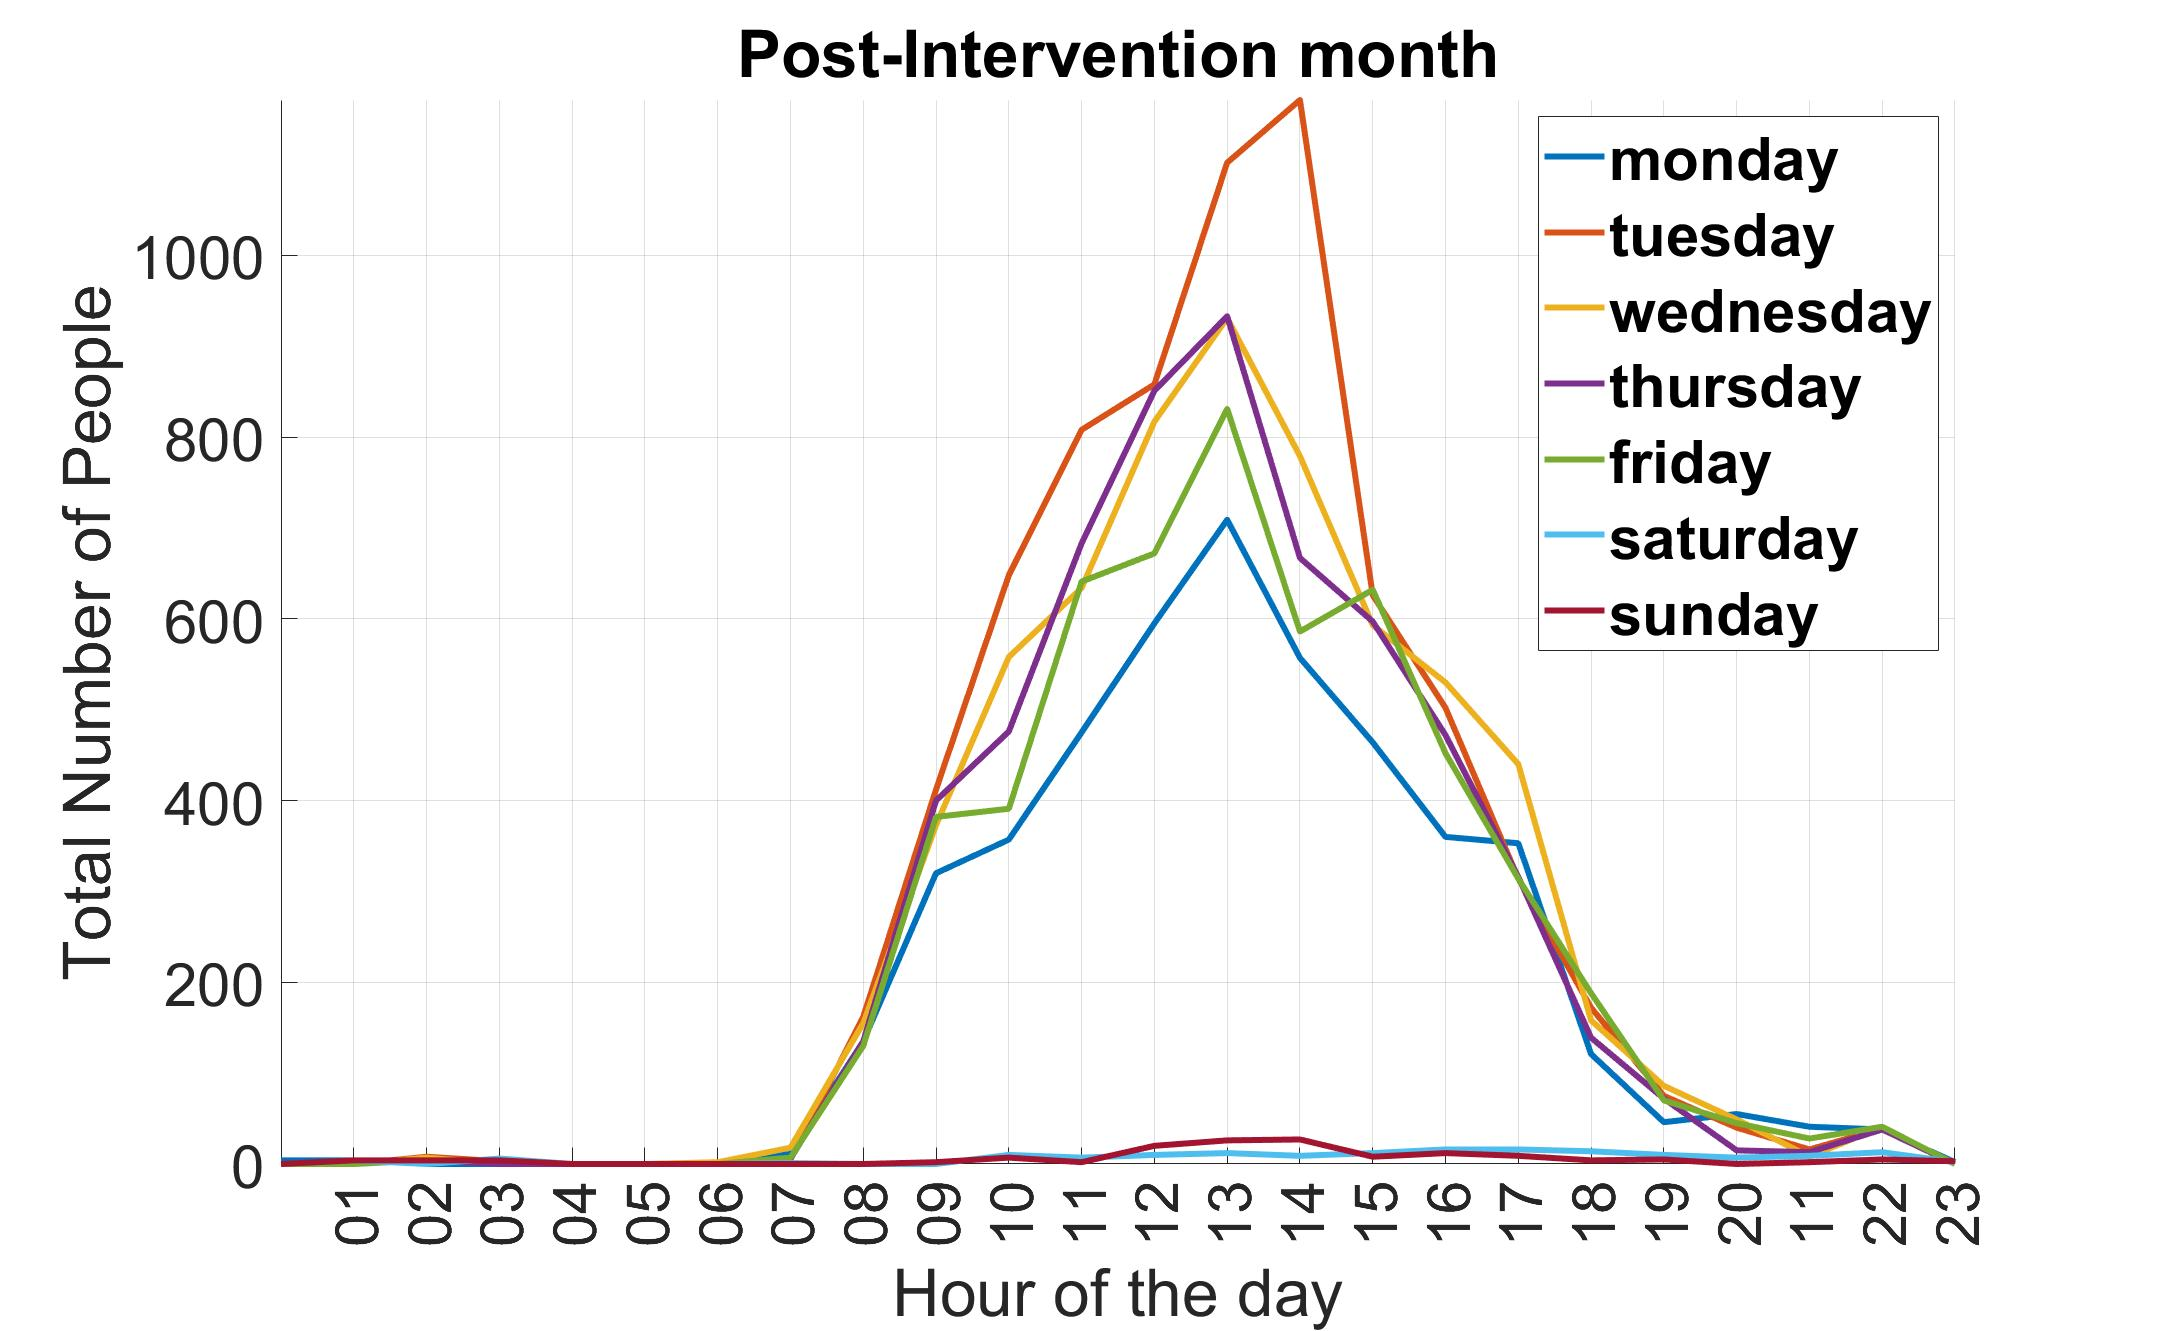
\includegraphics[width=.5\textwidth]{image/aggWeekPost.jpg}
    \\[\smallskipamount]
    \caption{Weekly distribution of the aggregated stair usage during the period of intervention.}
    \label{spa2}
\end{figure}




% change the visualization to include clusters(centroids and all data points)
\begin{figure}[!h]
\centering
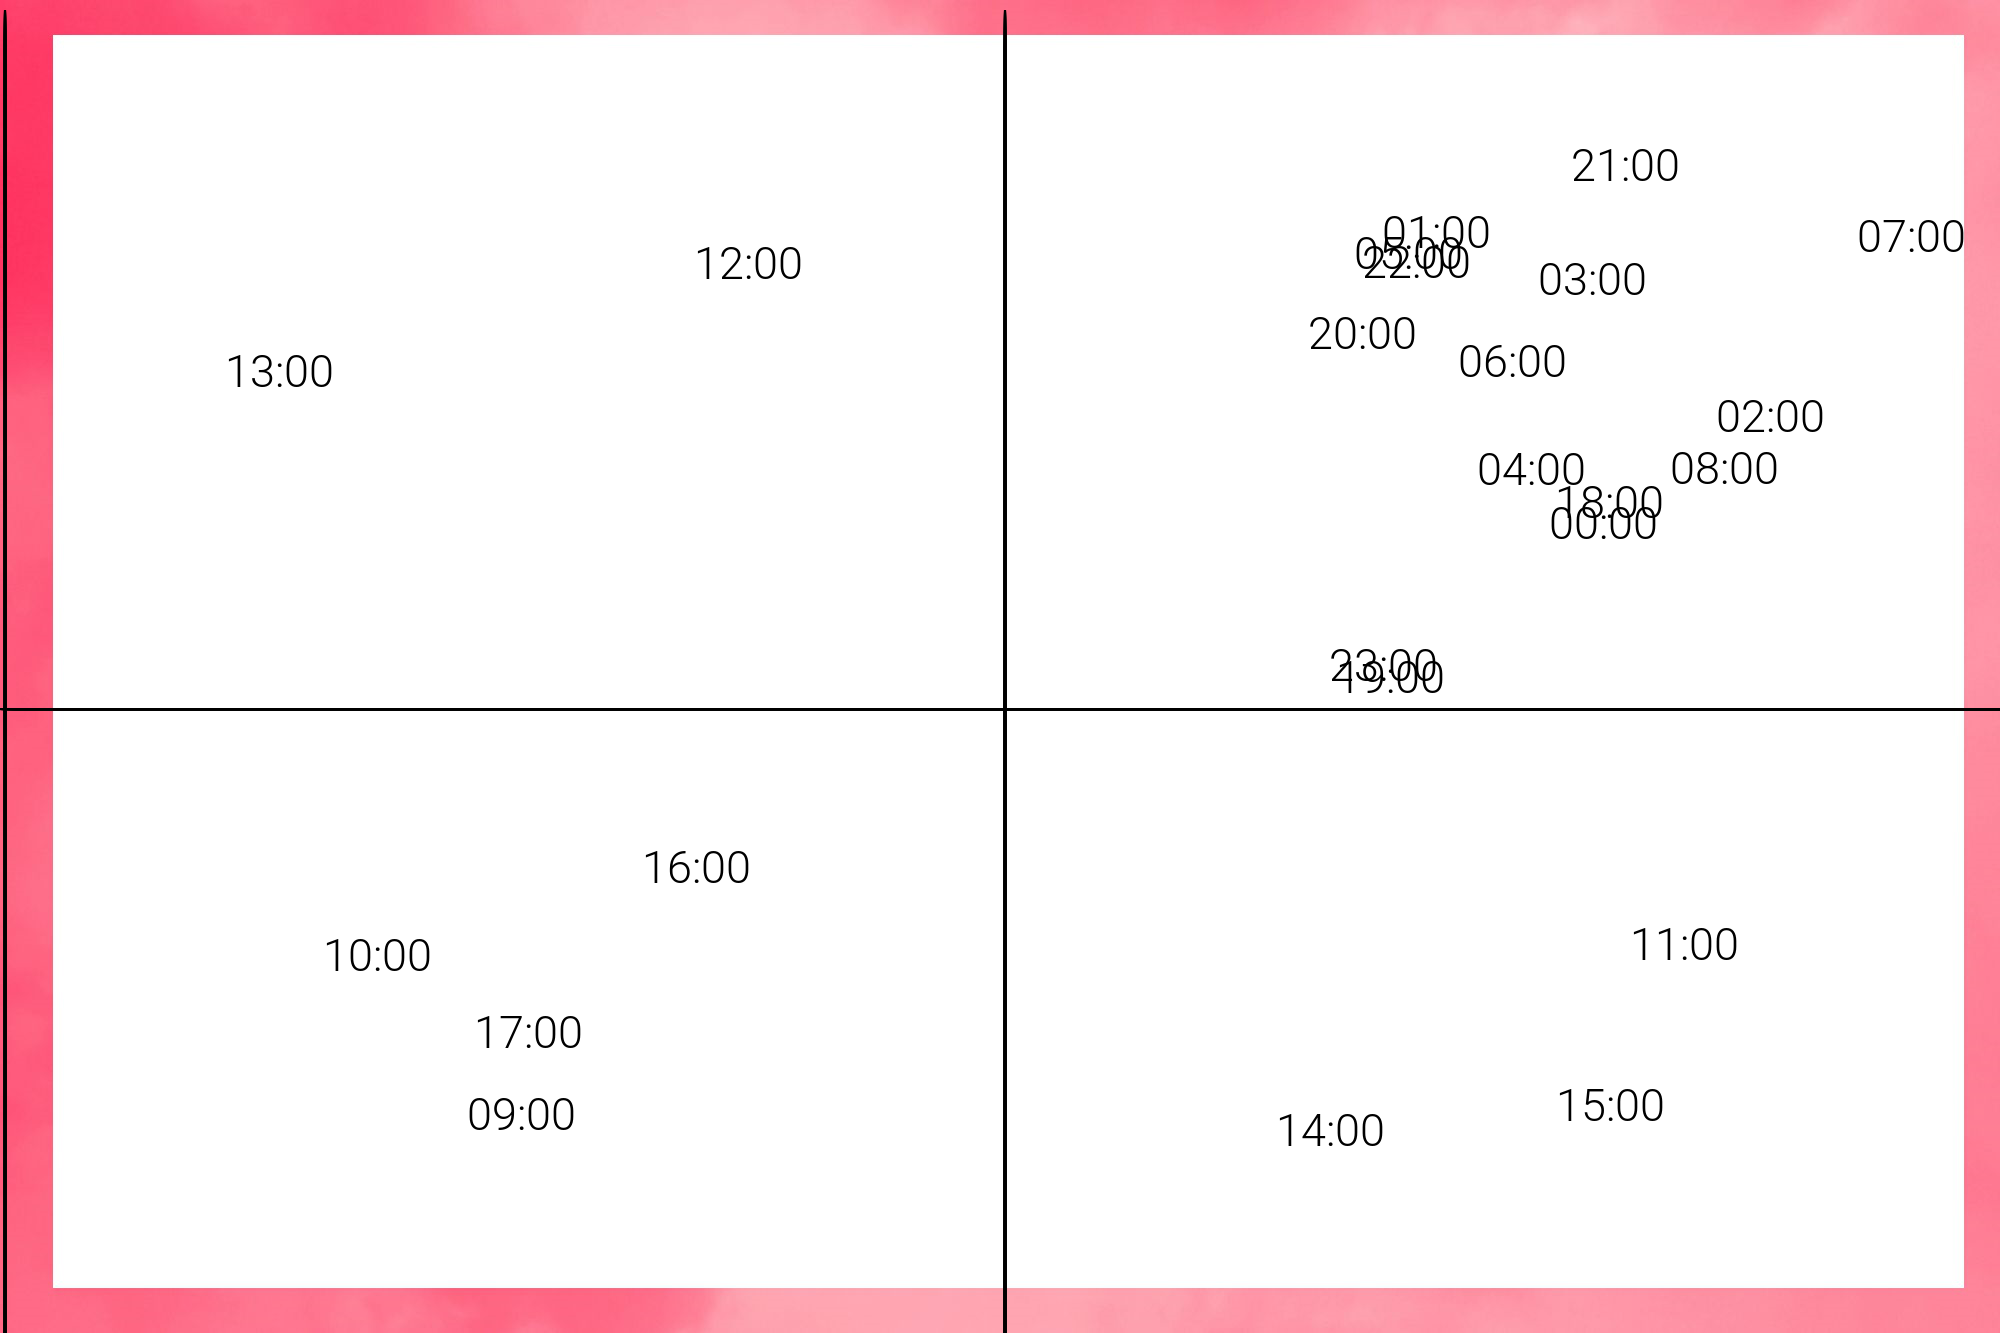
\includegraphics[width = 8cm,height = 7cm]{image/res.png}
\caption{Time series clustering: Hourly clustering of intervention month. It shows the similar times per days that have similar pattern. } 
\label{timegrup}
\end{figure}


    % \begin{figure}
    % \centering
    % 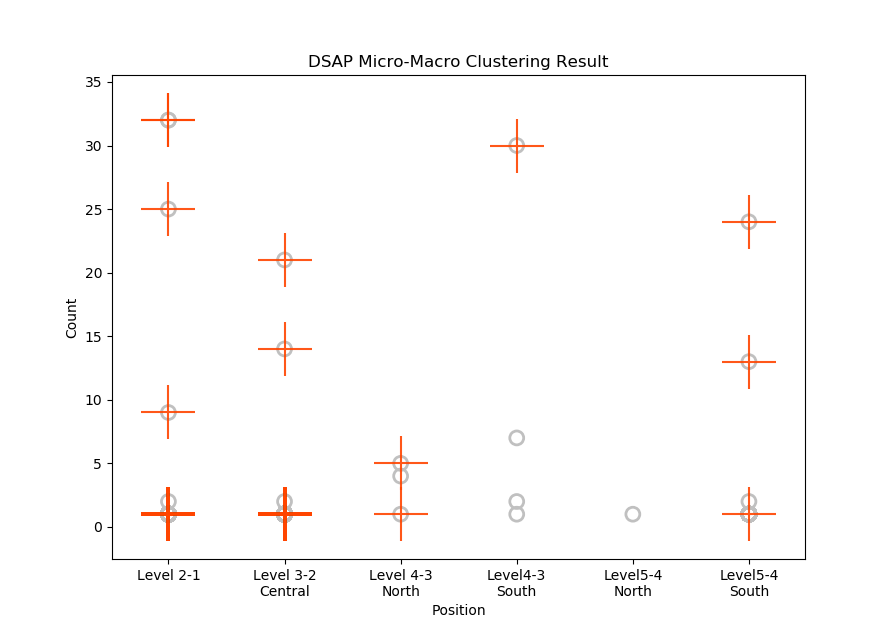
\includegraphics[width = 11 cm]{image/onemonth-threshold.png}
    % \caption{The DSAP result for the whole 3 month of experiment.}
    % \label{sci}
    % \end{figure}


\subsection{Clustering Algorithms}

The e-counter dataset is an example of spatially distributed measurements that could potentially be part of a continuous set of measurements. As the size of the data set increases, it soon becomes prohibitively expensive to analyze the entire data at a time. To find patterns in the data, clustering techniques are frequently employed. The e-counter experiment was performed to identify if any change in people's behavior was observed due to the active educational interventions that were made over a period of a month. The computer used in this study could only handle data for a week while performing the calculations required for the AP algorithm. The standard K-means algorithm is a much lighter algorithm and hence can handle the entire data set, but the cluster centers produced by K-means do not necessarily coincide with one of the data points. Hence for the sake of data interpretation, the K-means algorithm was not chosen as the primary tool for data analysis. Streaming K-means, in addition, needs an automatic estimation of the number of clusters which is not always straightforward in a data stream. In light of these issues, the streaming affinity propagation algorithm  DSAP was preferred for this study. But, for the sake of completeness and validation, the results from DSAP are compared with those from AP, k-means, and streaming K-means.    



    
Figure \ref{oneweek} shows the clusters generated by the AP algorithm for the first week of intervention from 29 April - 5 May, 2019. AP clustering algorithm, divided the dataXXX .
Based on the elbow method as shown in Figure \ref{elbkmean} left, the number of clusters seem to be six for this week. The corresponding clusters using k-means  are shown in the right of Figure \ref{elbkmean}. Explain clusters..xx Show k-mean centroid xxx
 




    
If the data comes in as a data stream or if the data is really large, then batch processing or stream clustering techniques can be applied to analyze the data. Employing a divide and conquer approach, the AP algorithm was applied using a one-hour landmark time window to compare against the results from AP and k-means for the first week of intervention starting on March 18. In order to interpret the results from the entire week more clearly, one needs to understand the evolution of clusters during a day. Some statistics from the first Wednesday of the intervention period are shown in Figure \ref{1daystat}. This day follows the overall pattern of stair usage as shown in the top-left panel of the Figure \ref{1daystat} which matches with the trends seen earlier in the aggregate plots \ref{spa2}. The accumulated number of people passing through a particular level is mentioned at the top of the panel shown in the top right of Figure \ref{1daystat}. This figure also shows the spatial distribution of measurements for the day. It should be noticed that levels 3-2 and 5-4 have similar aggregated numbers, but it seems like the contribution comes from a higher percentage of high value counts for level 5-4.

The bottom left panel of Figure \ref{1daystat} clearly shows that the maximum number of records measures only one person. Note that the scale of the y-axis is logarithmic and the number of records with higher count values reduces exponentially. The position histogram for the day is shown in the bottom-right of the same figure. On this day too the highest number of counts were observed on level 2-1 while both the north-side levels (4-3 North and 5-4 North) record the least activity that is at least three times lower than those of level 2-1. 

\begin{figure}[!h]
    \centering
   
    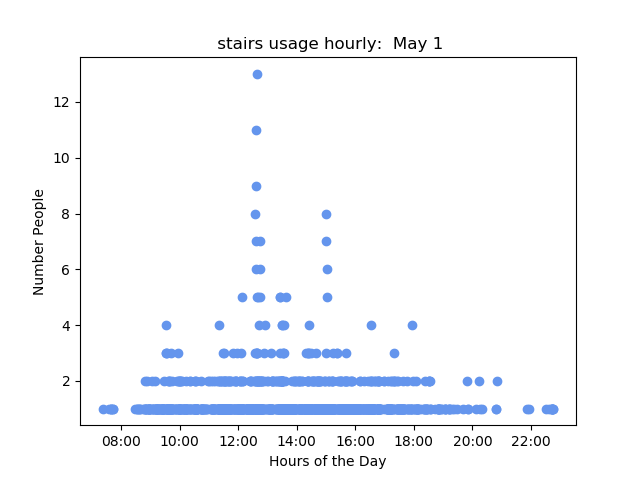
\includegraphics[width=0.5\textwidth]{image/Chapters/Chapter6/onedayhourMay1.png}\hfill
    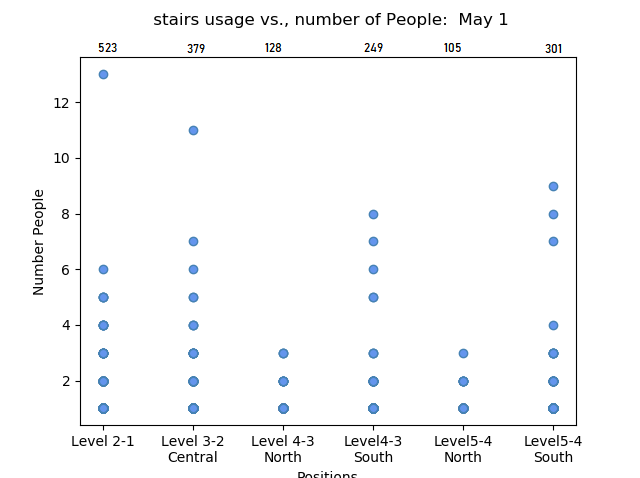
\includegraphics[width=0.5\textwidth]{image/Chapters/Chapter6/1day1monday1InterventionD.png}\hfill
    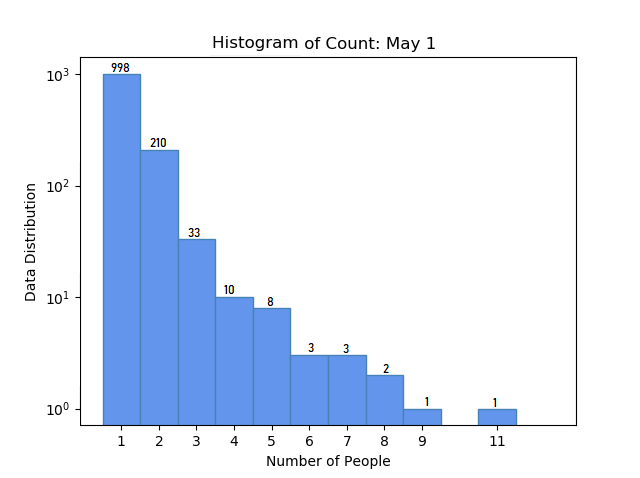
\includegraphics[width=0.5\textwidth]{image/Chapters/Chapter6/oneweekCountApril.png}\hfill 
    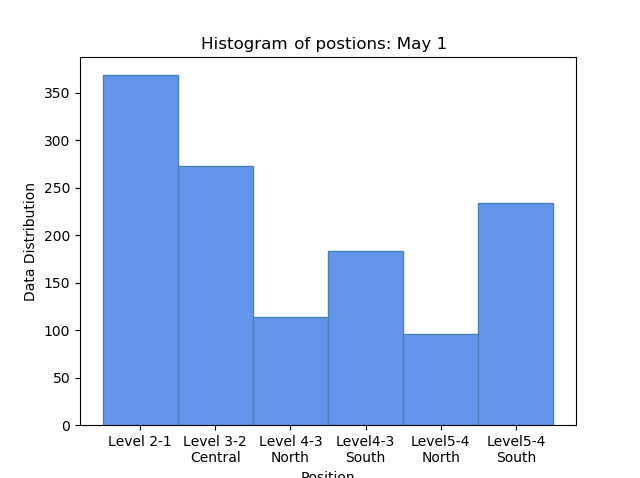
\includegraphics[width=0.5\textwidth]{image/Chapters/Chapter6/oneweek(Monday)Hist.png}
    \caption{One day data distribution. First Wednesday of intervention: May 1. Top left- The total count of people at all the levels during the entire day starting at 7 a.m. Top right- The measured count of people at each level for the day. Bottom left- Histogram of the people count registered at all levels. Bottom right- Histogram of the measurements made at each level for the day }
    \label{1daystat}
\end{figure}

######## RESULts from AP only: hourly and weekly
Data from May 1 were split in one hour landmark window time windows and analyzed using a divide and conquer approach with the AP algorithm to generate micro-clusters. The clusters obtained during each hour from 7 am to 7 pm along with the branch points of each cluster are shown in Figure \ref{AP1}. The evolution of people activity across all levels can be clearly seen from these plots. The clusters capture the increase in activity starting around 9-11 am xxxxxxx
% \begin{figure}[!h]
%     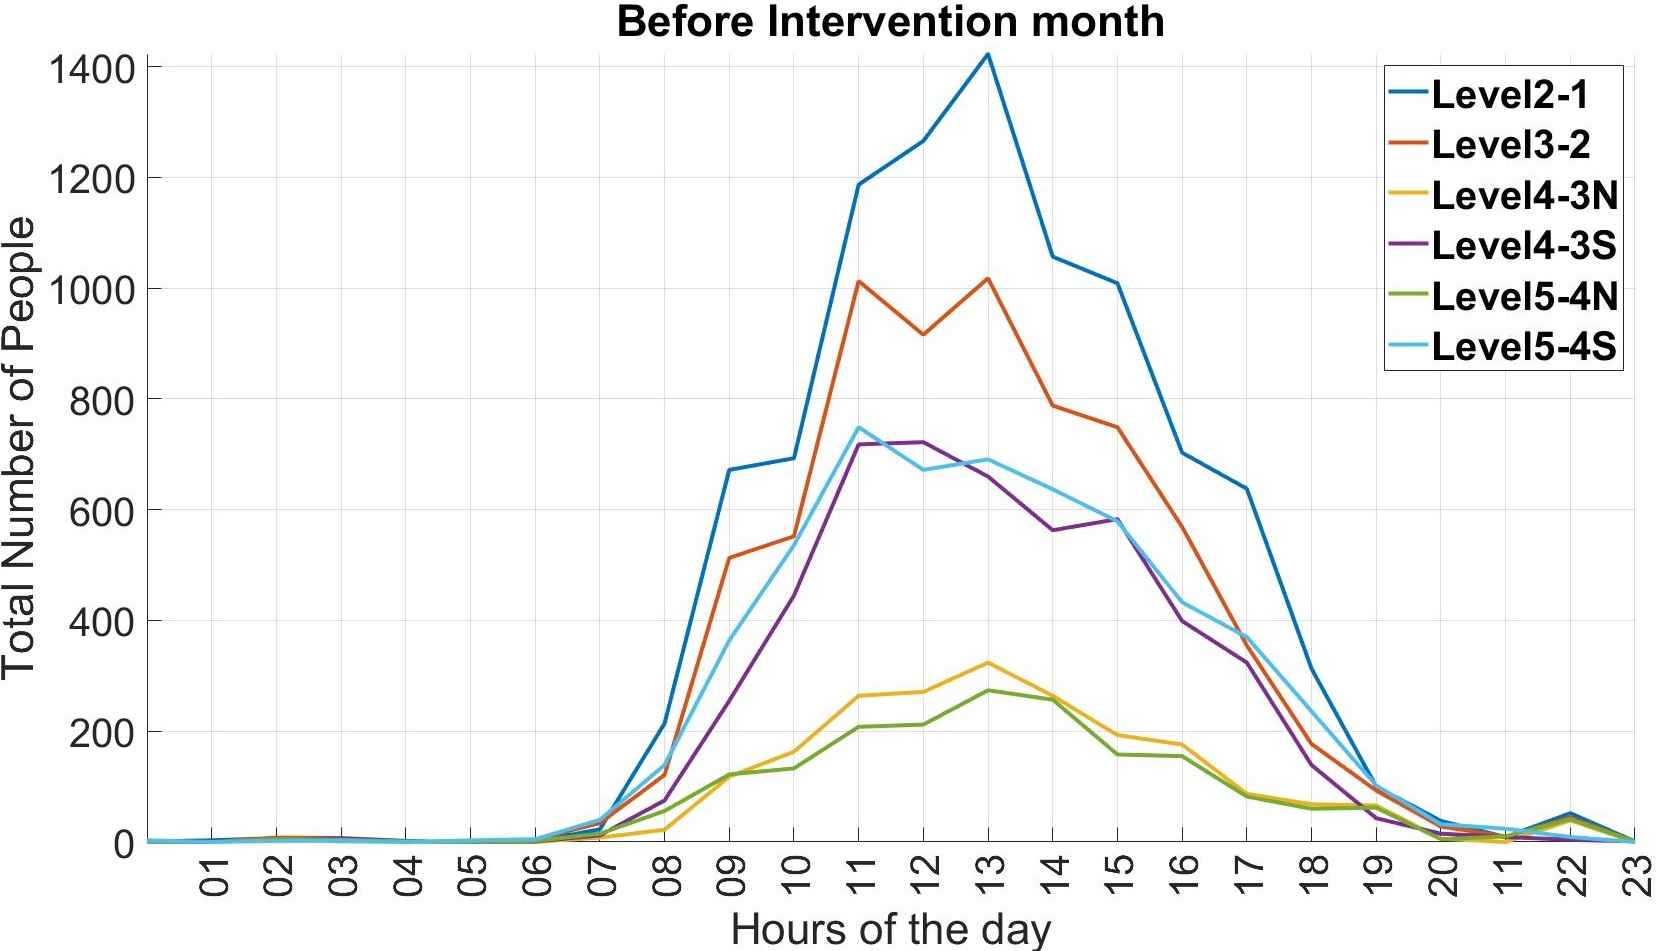
\includegraphics[width=.5\textwidth]{image/before_int.jpg}\hfill
%     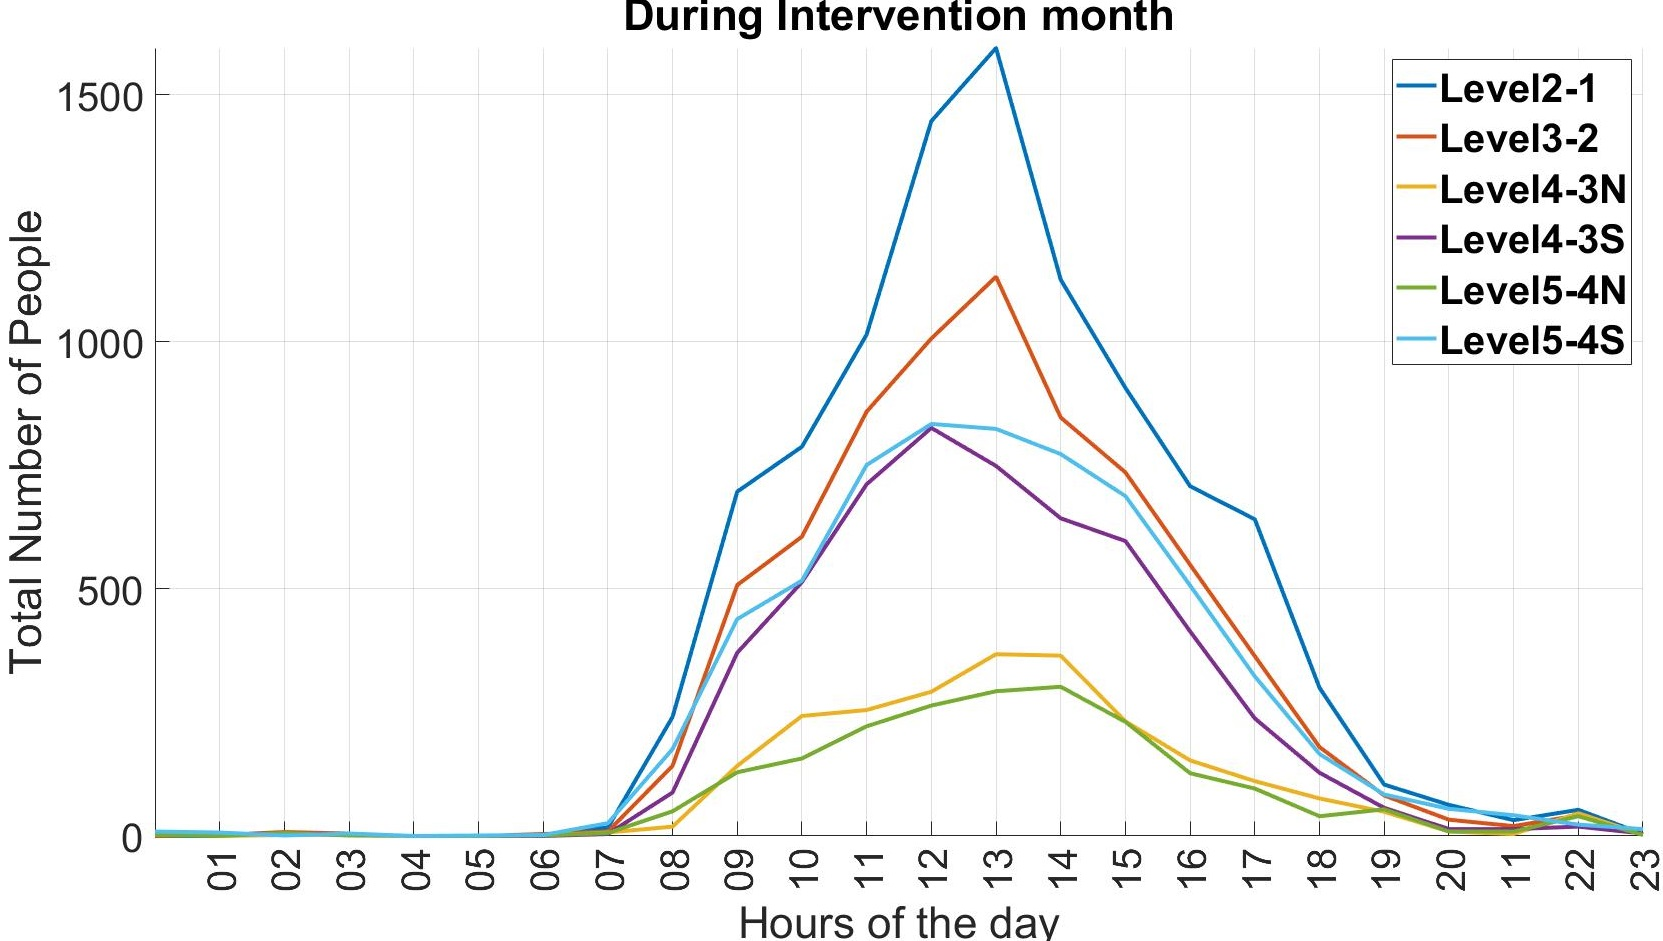
\includegraphics[width=.5\textwidth]{image/during_int.jpg}\hfill\centering
%     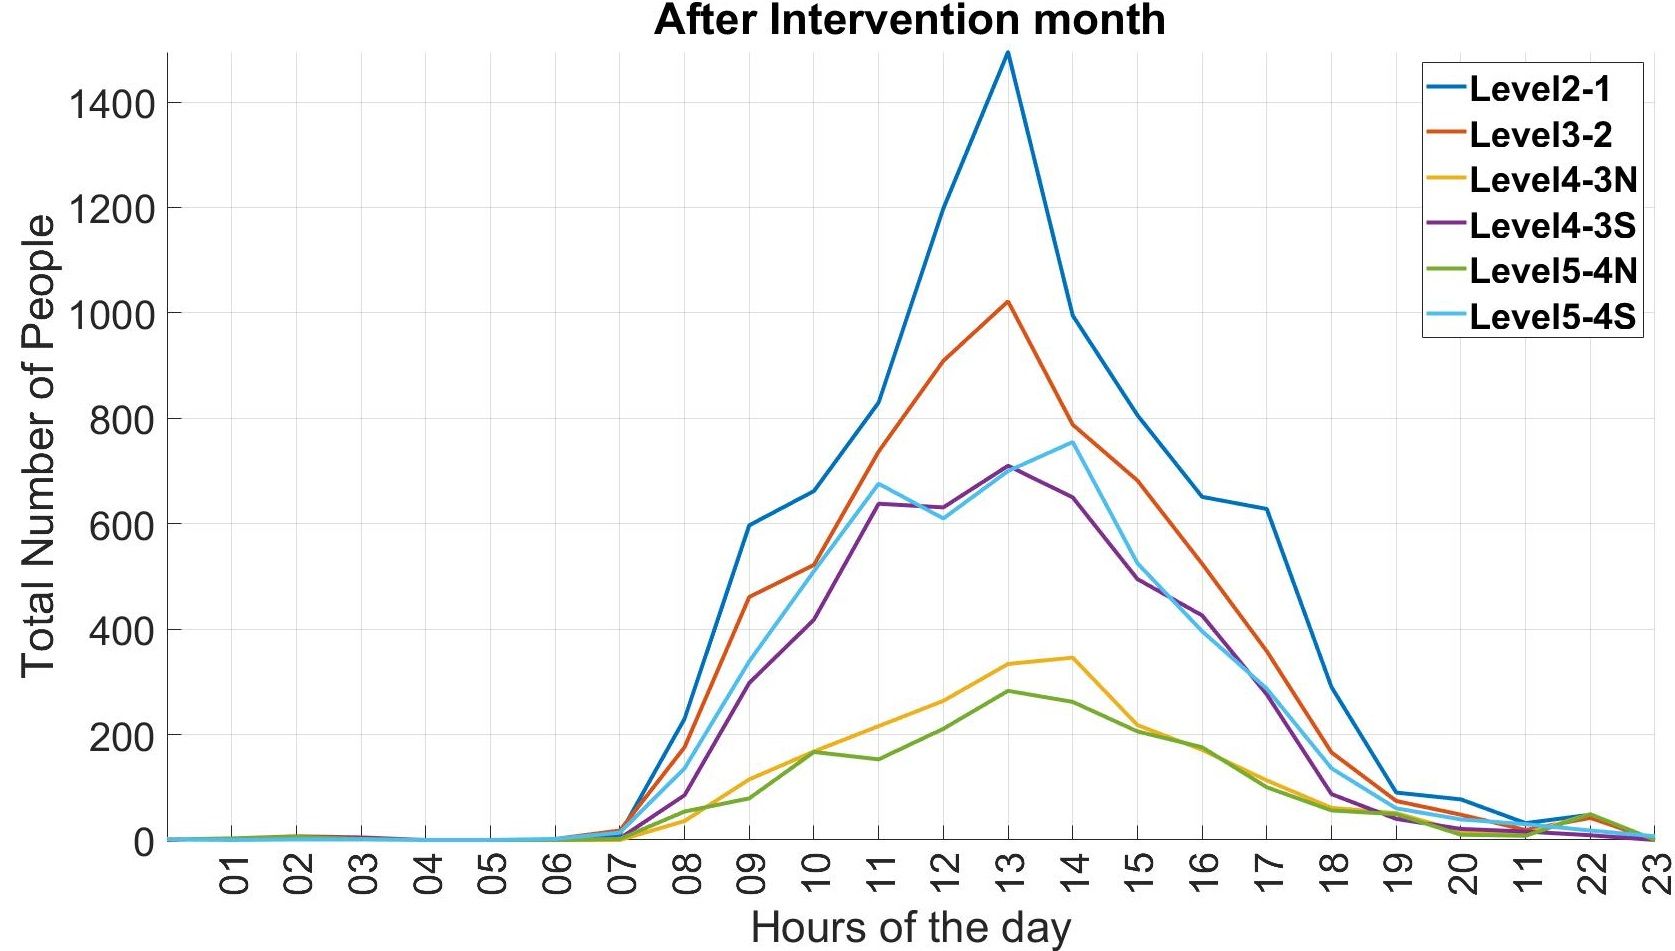
\includegraphics[width=.5\textwidth]{image/after_int.jpg}
%     \\[\smallskipamount]
%     \caption{Spatio-temporal distribution of the aggregated stair usage during the period of intervention.}
%     \label{spa1}
% \end{figure}




\begin{figure}[htp]
%\centering
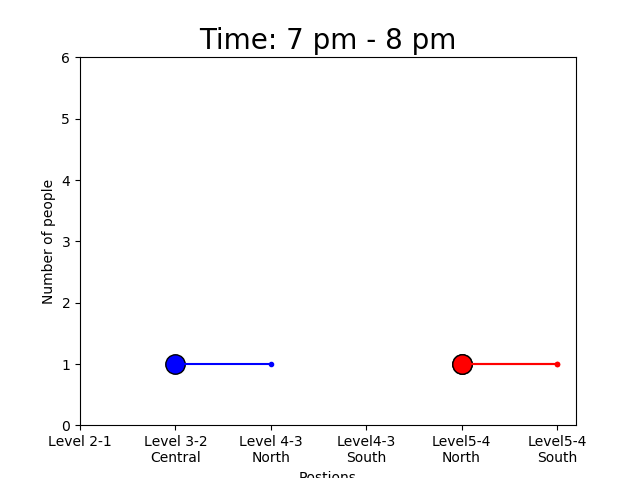
\includegraphics[width=.33\textwidth]{image/Chapters/Chapter6/7.png}%\quad
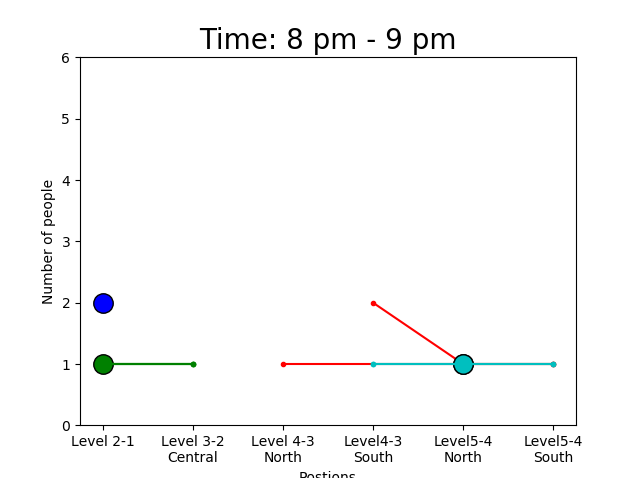
\includegraphics[width=.33\textwidth]{image/Chapters/Chapter6/8.png}%\quad
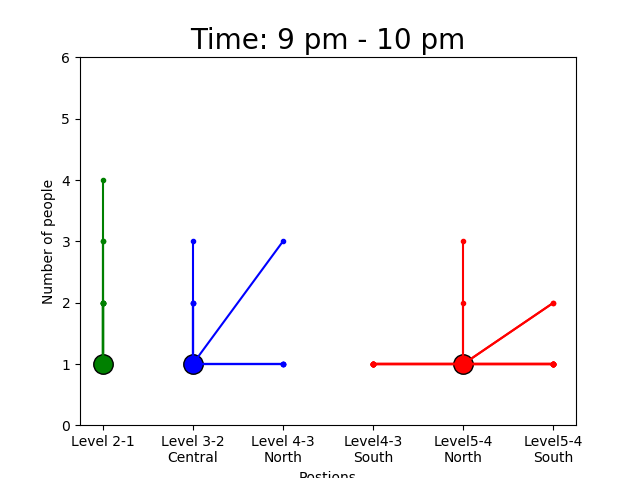
\includegraphics[width=.33\textwidth]{image/Chapters/Chapter6/9.png}

% \medskip

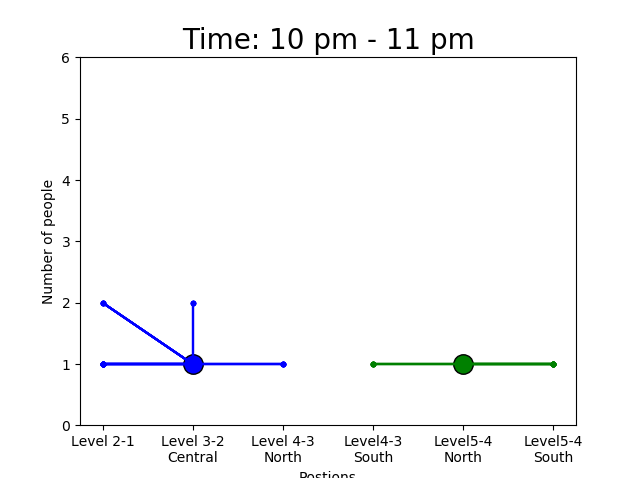
\includegraphics[width=.33\textwidth]{image/Chapters/Chapter6/10.png}%\quad
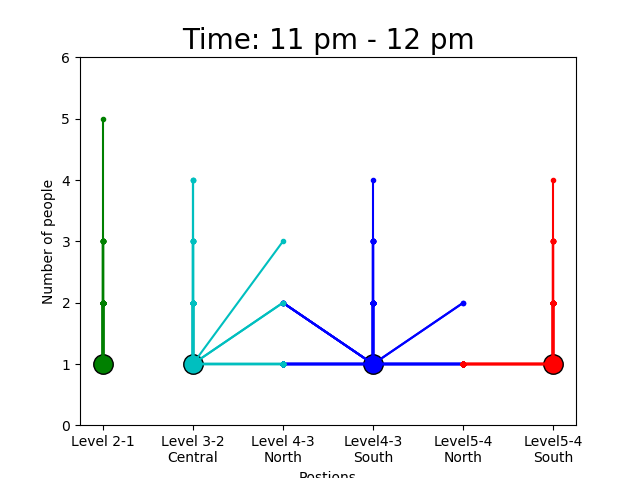
\includegraphics[width=.33\textwidth]{image/Chapters/Chapter6/11.png}%\quad
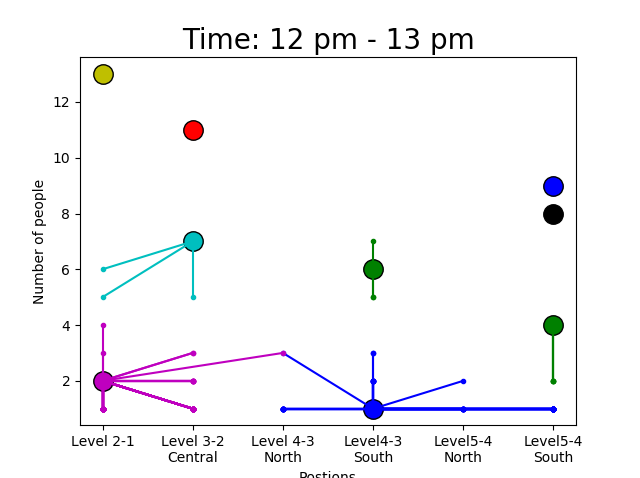
\includegraphics[width=.33\textwidth]{image/Chapters/Chapter6/12.png}

% \medskip

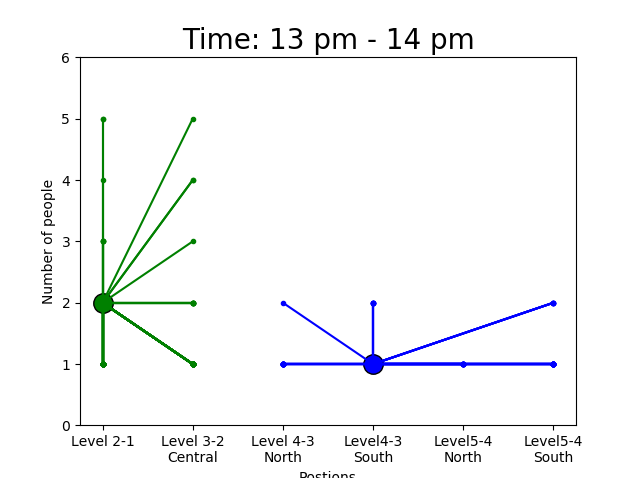
\includegraphics[width=.33\textwidth]{image/Chapters/Chapter6/13.png}%\quad
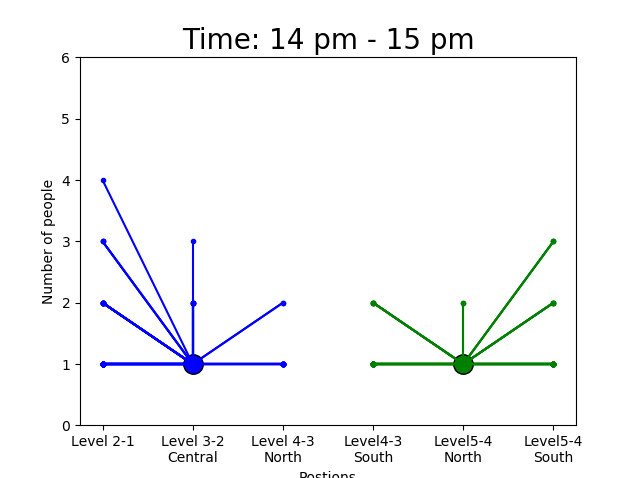
\includegraphics[width=.33\textwidth]{image/Chapters/Chapter6/14.png}%\quad
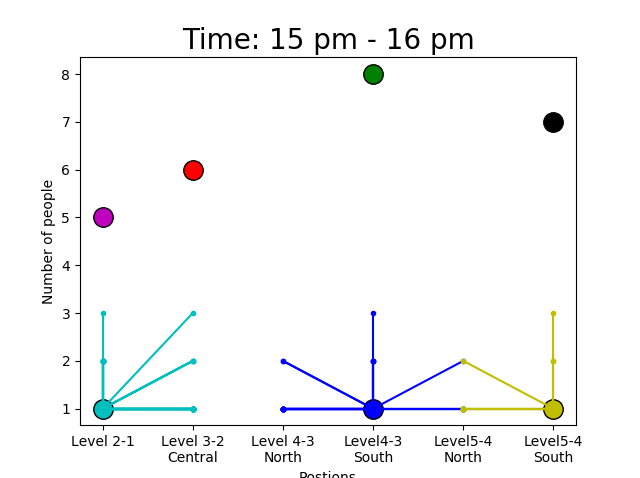
\includegraphics[width=.33\textwidth]{image/Chapters/Chapter6/15.png}
% \medskip

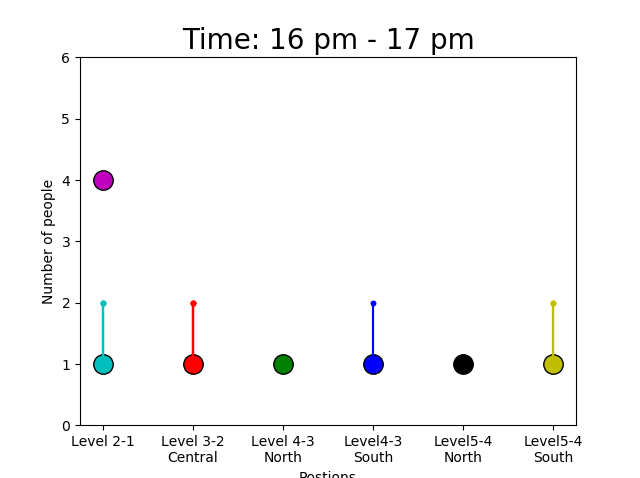
\includegraphics[width=.33\textwidth]{image/Chapters/Chapter6/16.png}%\quad
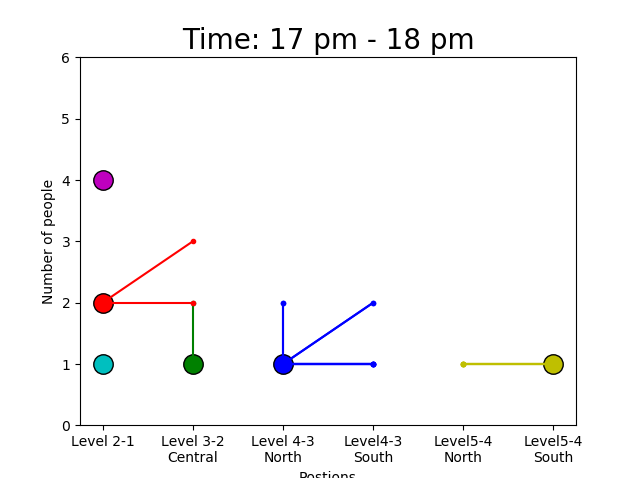
\includegraphics[width=.33\textwidth]{image/Chapters/Chapter6/17.png}%\quad
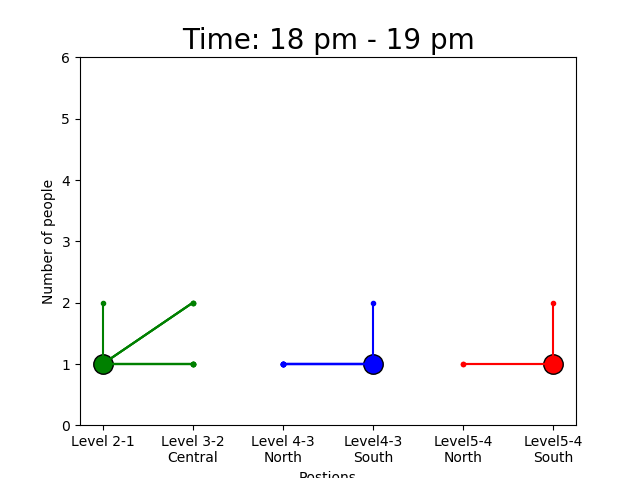
\includegraphics[width=.33\textwidth]{image/Chapters/Chapter6/18.png}

\caption{Affinity propagation clustering Algorithm with the number of people at different stairs for each hour with landmark time window between 7 am to 7 pm on Wednesday May 1, 2019, first week of intervention month. Early Hours Clusters; Mid-Morning; Lunch-time Hourly; Afternoon time}
\label{AP1}
\end{figure}
%%%%%%%%%%%%%%%%%%%%%%%%%%%%%%%%%%%%%%%%%%%%%%%%%%%%%%%%%%%
% The entire time evolution of the cluster centres for the week is concisely represented in Figure. \ref{week3d}. XX %Maybe the macro cluster plot from dsap V1 for one week here ? XX



% \begin{figure}
% \centering
% 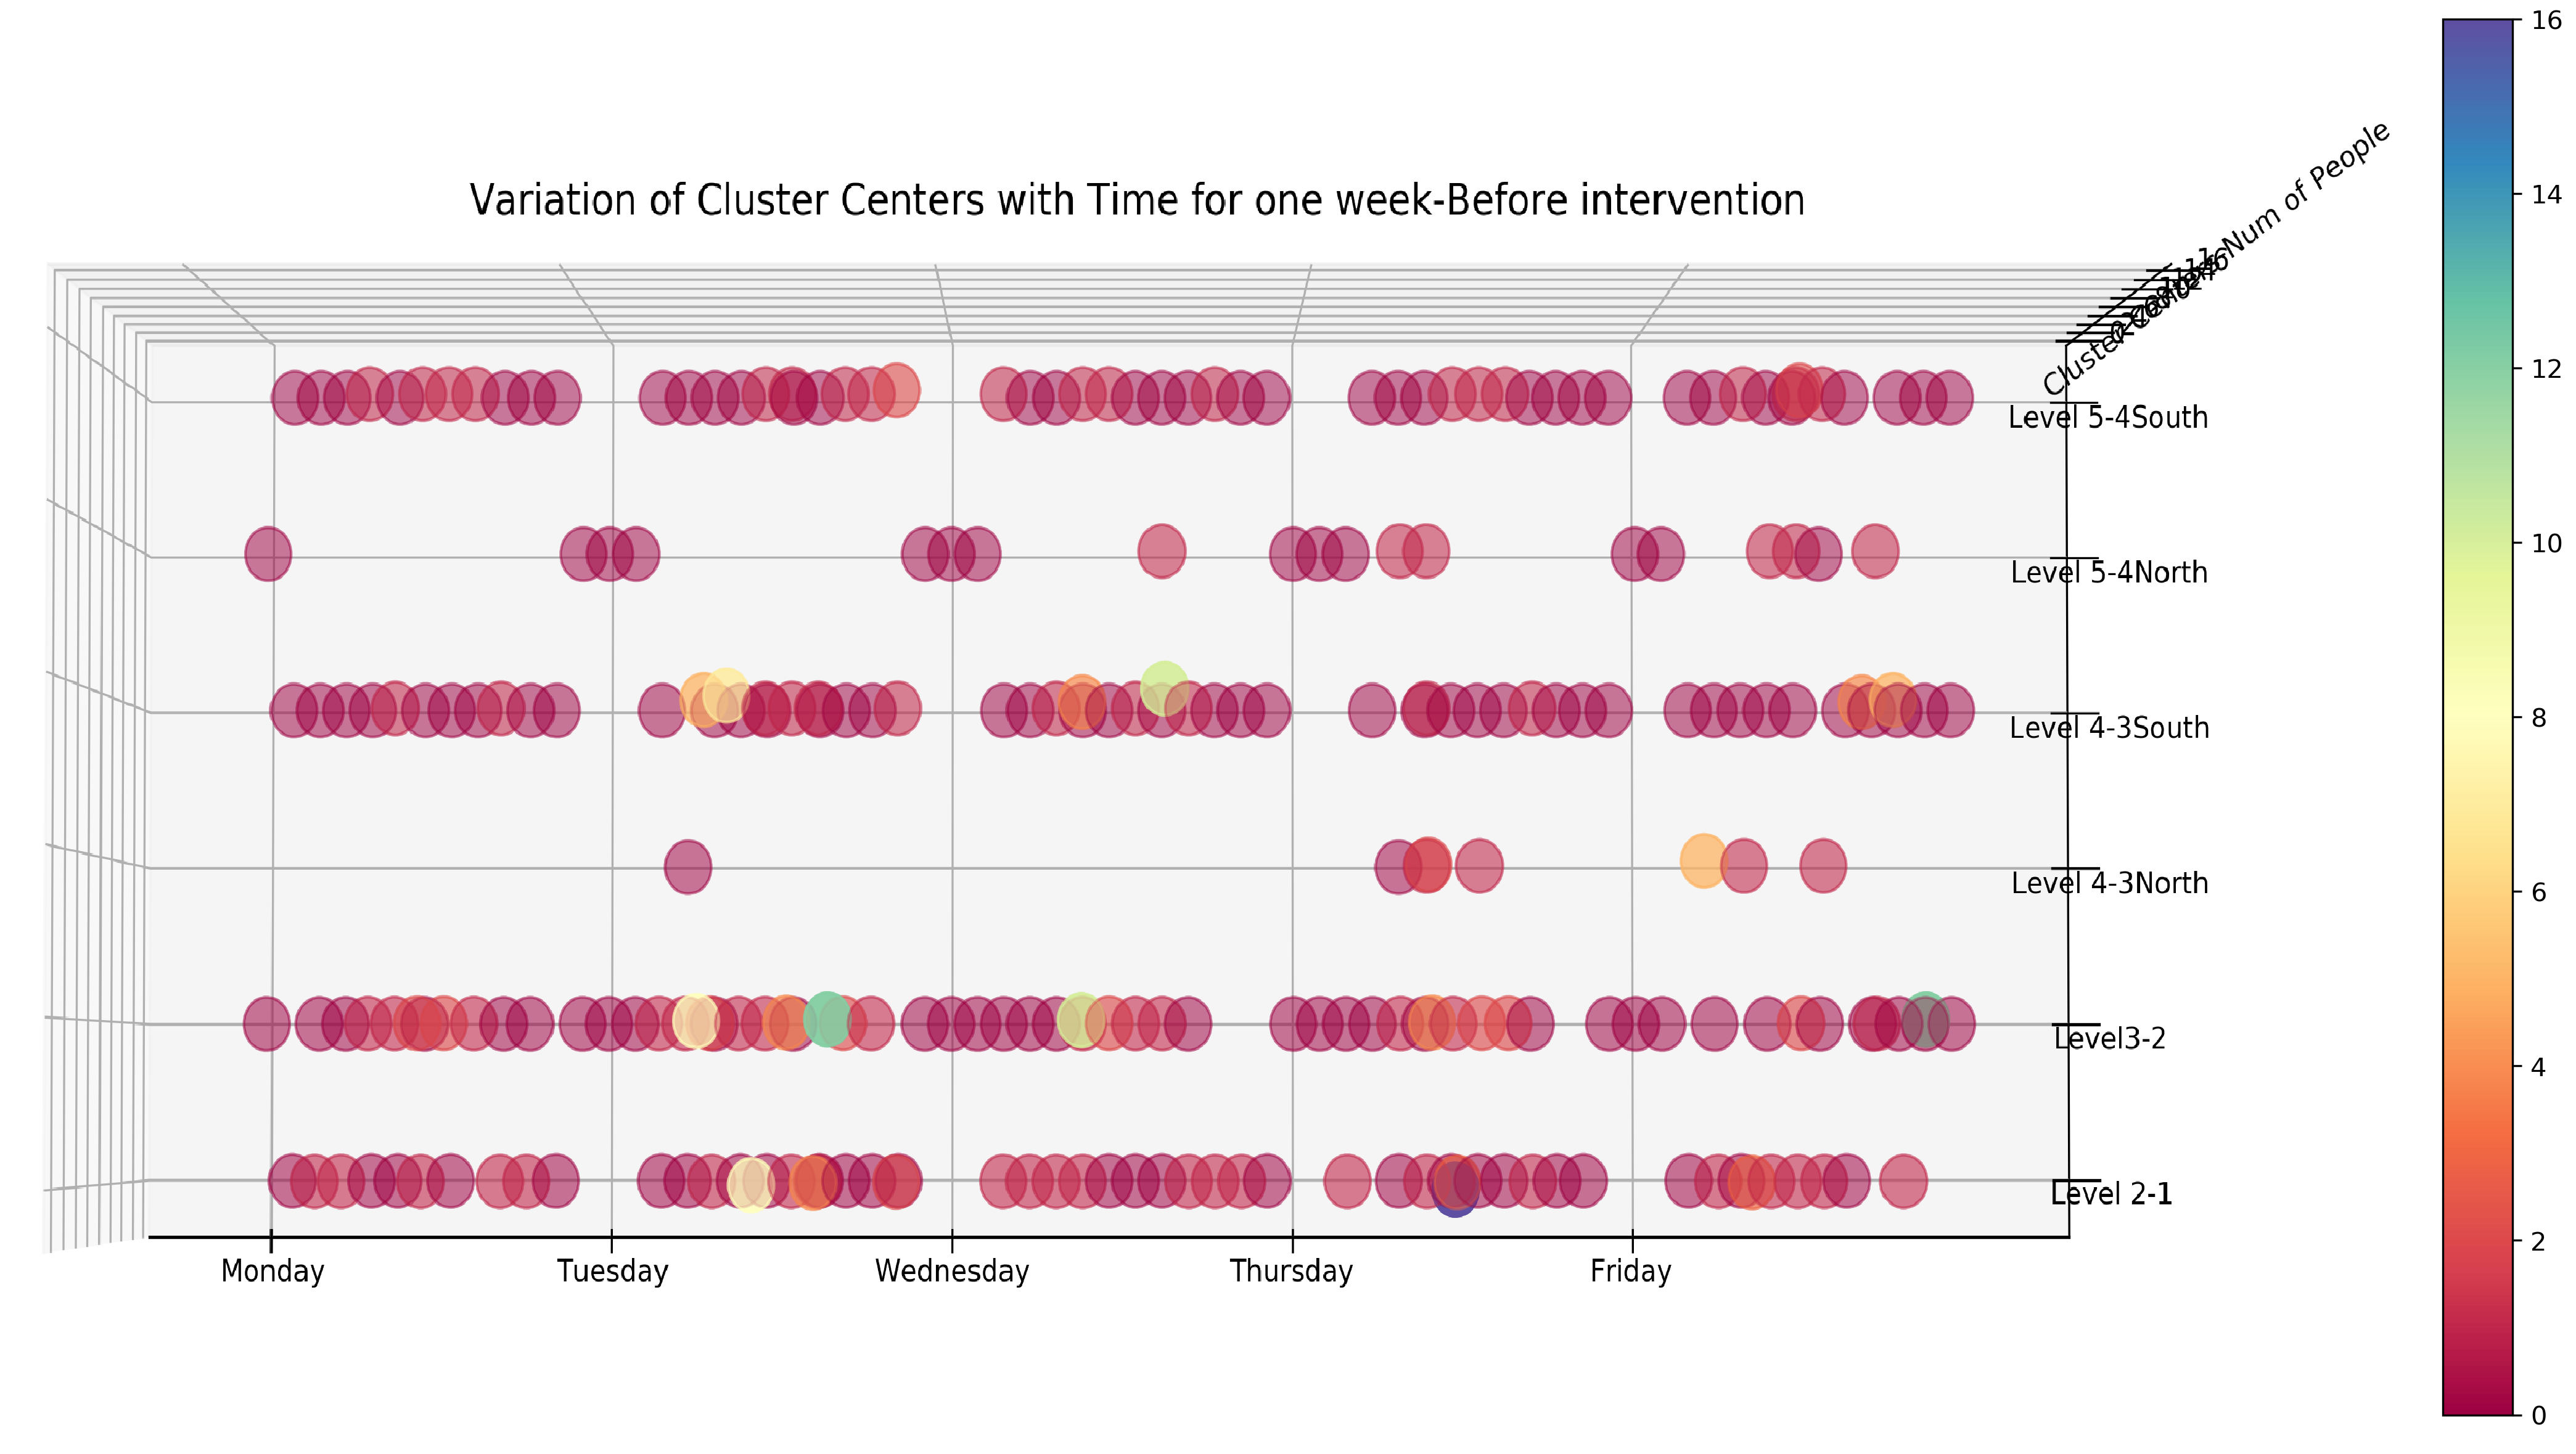
\includegraphics[width = 10cm,height = 7cm]{image/ClusterCentCount_3.png}
% \caption{ The evolution of the cluster centres from 8am - 7 pm during the first week of intervention from April 29 - May 5.}
% \label{week3d}
% \end{figure}

%%%%%%%%%%%%%%%% One day summary
%%%%%%%%%%%%%%%% one week LBAP cluster evolution
%%%%%%%%%%%%%%% one week LBAP macro miicro
%%%%%%%%%%%%%%%%%%%%%%%%%%%%%%%%%%%%%%%%%%%%%%%%%%%%%%%%%%%%%%

The first week of intervention was also analyzed using a 4 hour landmark time window. It was found out that using 4 hours gave optimum cluster values since the first time window needs to have a critical number of points to initialize the process. All the micro clusters generated during the week are plotted as blue circles while the macro clusters are shown as red crosses. (Explain clusters XX). These results can be compared with the clusters generated by AP and K-means for the same week shown earlier in Figures. \ref{oneweek} and \ref{elbkmean}. To compare the results from these three techniques, the internal and external evaluation metrics are compiled in Table \ref{all3}. The significant savings in time is immediately apparent between the DSAP algorithm and AP. For a real stream the calculation time for a window is expected to be lower in DSAP as the initial window calculation that is the most time intensive step is performed once and doesn't affect the current time window. The accuracy of the two methods is still similar as reported by the other metrics. % Why isn't the memory lower?  














%%%%%%%%%%%%%%%%%%%%%%%%%%%%%%%%%%%%%%%%%%%%%%%%%%%%%%%%%%%%%%%%%%%%%% Before Intervention


\begin{figure}[!h]
    \centering
    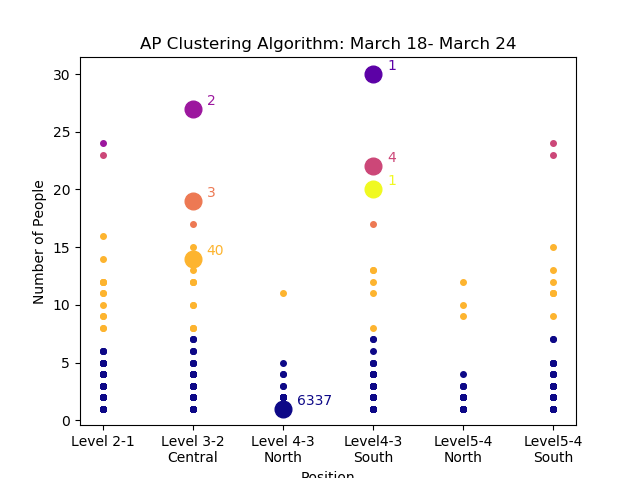
\includegraphics[width = 11 cm]{image/Chapters/Chapter6/ApFirstWeekBeforeInt.png}
    \caption{AP algorithm is applied on e-counter data for one week. The first week before intervention. with the damping = 0.96 and preference(np.median(similarity matrix) = -4 }
    \label{befA}
\end{figure}



\begin{figure}[!h]
    \centering
    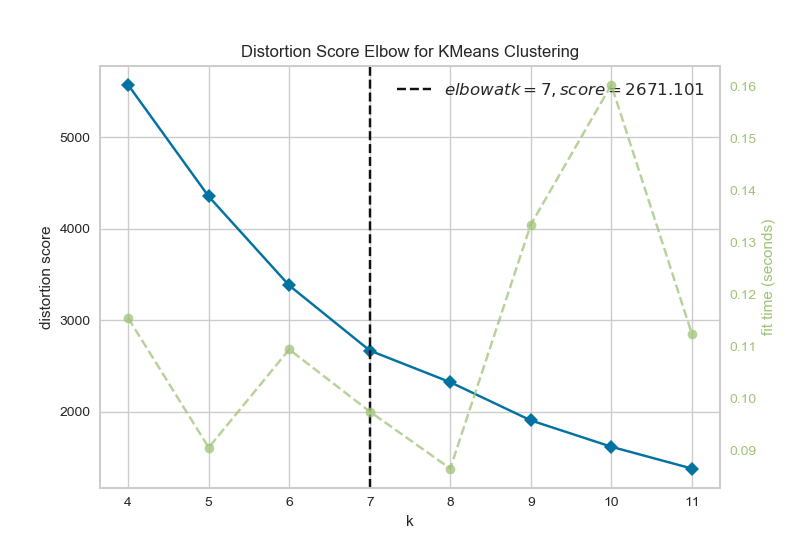
\includegraphics[width=.49\textwidth]{image/Chapters/Chapter6/elbowBeforerInt.png}
    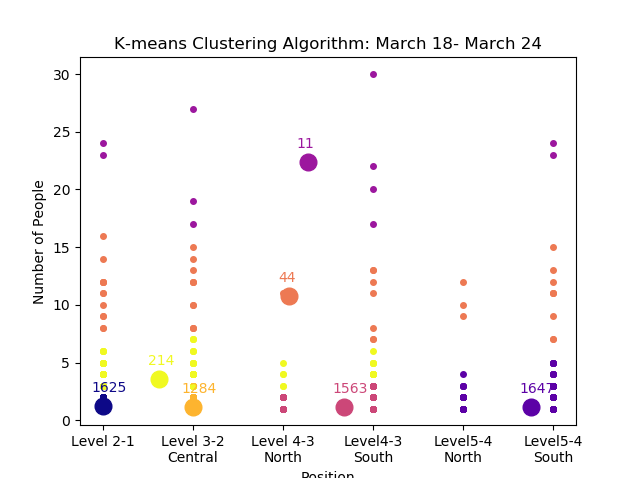
\includegraphics[width=.49\textwidth]{image/Chapters/Chapter6/kmeans1WeekBefore.png}
    \caption{K-means algorithm is applied on e-counter data for one week(first week before intervention: March 18- March 24).}
    \label{beforAPp}
\end{figure}   
   




\begin{figure}[]
    \centering
    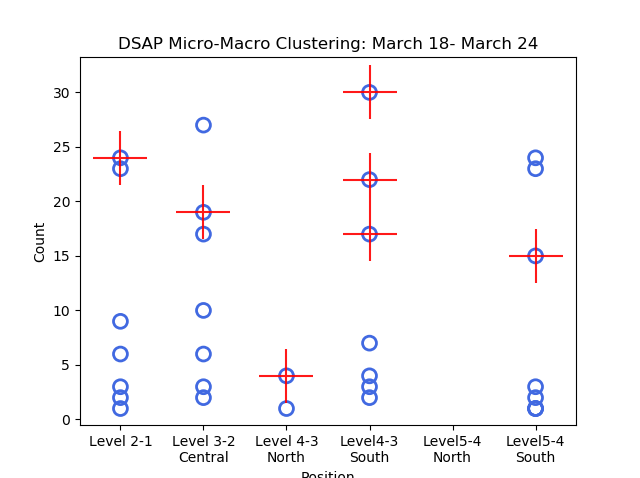
\includegraphics[width=.49\textwidth]{image/Chapters/Chapter6/before5hour-samp 9.preference 4.No Thre.png}%ecounter_time data
    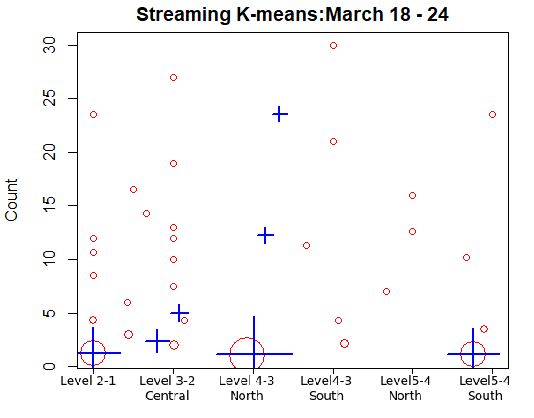
\includegraphics[width=.49\textwidth]{image/Chapters/Chapter6/streamKbefore1.png}
    \caption{Clustering results from DSAP and streaming K-means algorithms applied on the e-counter data for the first week before intervention. damping = 0.9, expiration value = 50.}
    \label{26}
\end{figure}




\begin{figure}[!h]
    \centering
      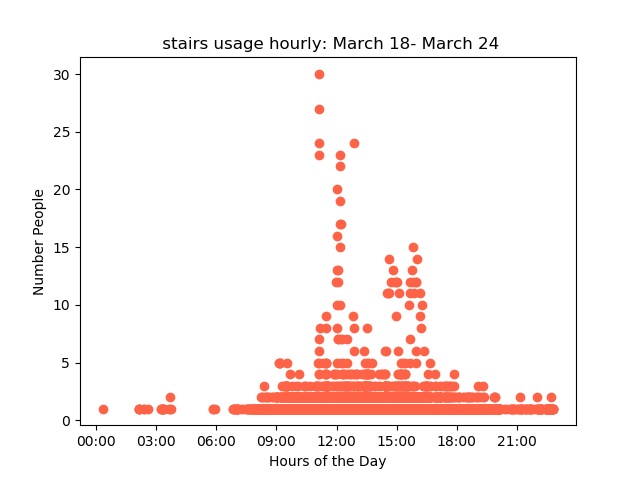
\includegraphics[width=0.5\textwidth]{image/Chapters/Chapter6/oneWeekBeforehourly.png}\hfill
    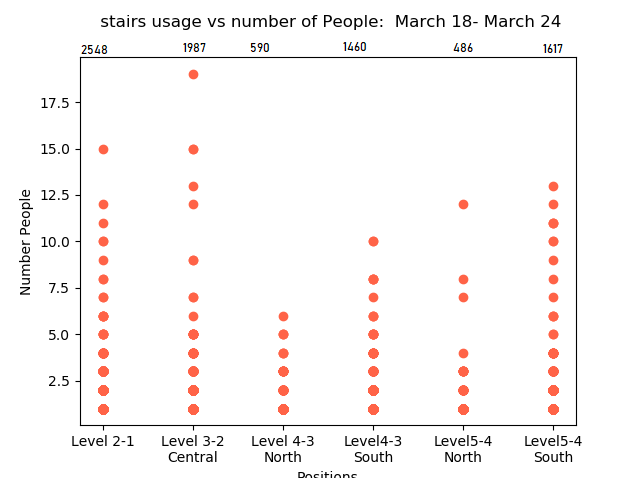
\includegraphics[width=0.5\textwidth]{image/Chapters/Chapter6/PositionCountOneWeekBeforer.png}\hfill
    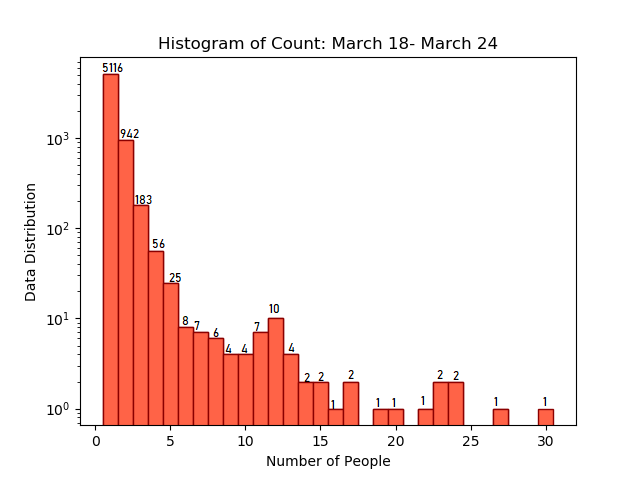
\includegraphics[width=0.5\textwidth]{image/Chapters/Chapter6/oneweekCountDistributonBefore.png}\hfill 
    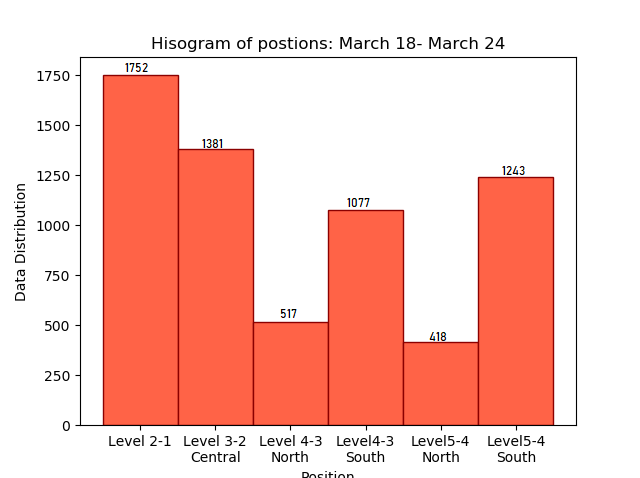
\includegraphics[width=0.5\textwidth]{image/Chapters/Chapter6/oneweekBeforePositionDistributon.png}
    \caption{One week data distribution. First week before intervention from March 18 - March 24.}
    \label{55}
\end{figure}




\begin{table}[!h]
\small
\caption{Comparison of AP, DSAP, K-means, and Streaming K-means Evaluation Metrics for the first week before intervention ( March 18- March 24).}
\label{befcom}
\begin{tabular}{l
>{\columncolor[HTML]{CBCEFB}}c 
>{\columncolor[HTML]{FFCCC9}}c 
>{\columncolor[HTML]{CBCEFB}}c 
>{\columncolor[HTML]{FFCCC9}}c }
\hline
\multicolumn{1}{c}{\textbf{Metrics}} & \textbf{AP} & \textbf{K-means} & \textbf{DSAP} & \textbf{Stream K-means} \\ \hline\midrule
\textbf{Processing time (s)}         & 23          & 0.28             & 0.66           & 0.6                       \\ \hline
\textbf{Memory consumption (MB)}     & 517         & 580              & 212           & 313                        \\ \hline
\textbf{Number of clusters}          & 7           & 7                & 7             & 7                          \\ \hline
\textbf{Silhouette Index}      & 0.7         & 0.6              & 0.5         & 0.7                       \\ \hline
\textbf{Caliński-Harabasz Index}     & 380         & 1237             & 87            & 150                         \\ \hline
\textbf{Davies-Bouldin Index}        & 0.6         & 0.5              & 0.5          & 0.19                        \\ \hline\midrule
\end{tabular}
\end{table}

    




%%%%%%%%%%%%%%%%%%%%%%%%%%%%%%%%%%%%%%%%%%%%%%%%%%%%%%%%%%%%%%%%%%%%%%  During Intervention
\begin{figure}[!h]
    \centering
    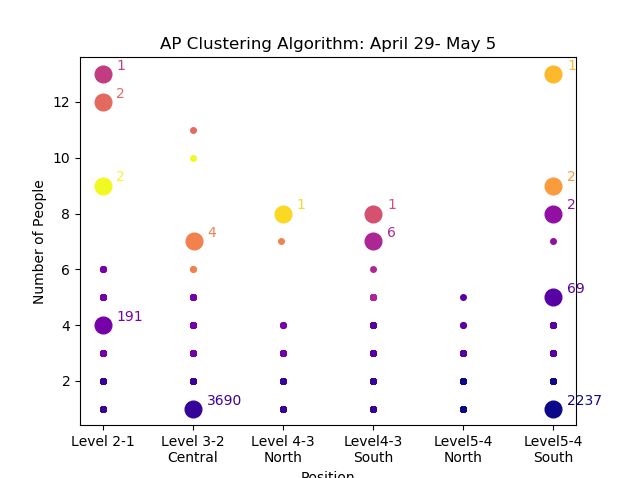
\includegraphics[width = 11 cm]{image/Chapters/Chapter6/ApFirstWeekIntervention1.png}
    % 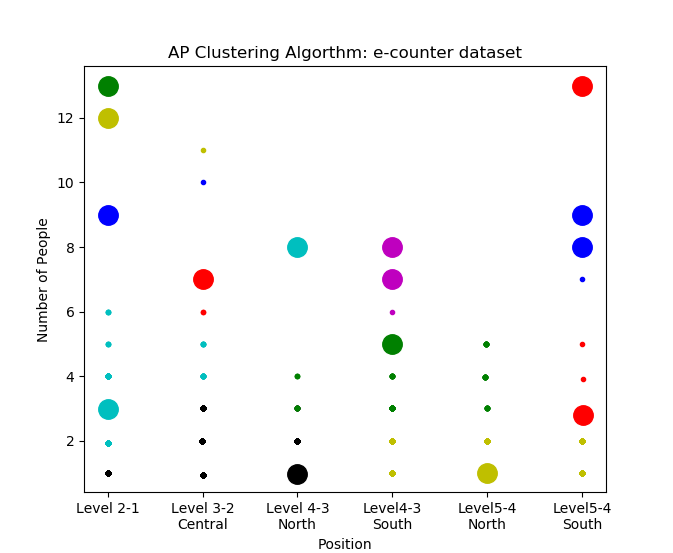
\includegraphics[width = 11 cm]{image/Chapters/Chapter6/17ap.966Y.png}%ecounter_time data
    \caption{AP algorithm is applied on e-counter data for one week. The first week of intervention: 29 April- 5 May. with the damping = 0.96 and preference(np.median(similarity matrix) = -50 }
    \label{oneweek}
\end{figure}

    
\begin{figure}[!h]
    \centering
    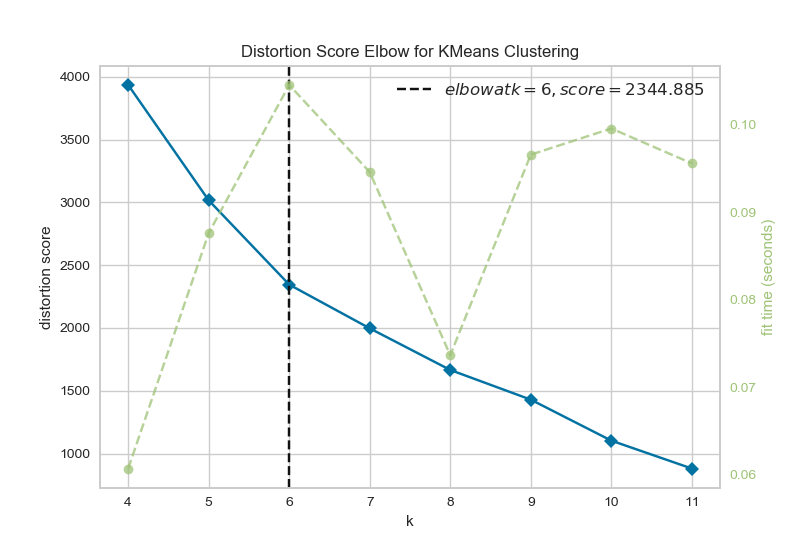
\includegraphics[width=.5\textwidth]{image/Chapters/Chapter6/elbow.png}%29apriloneweek data
    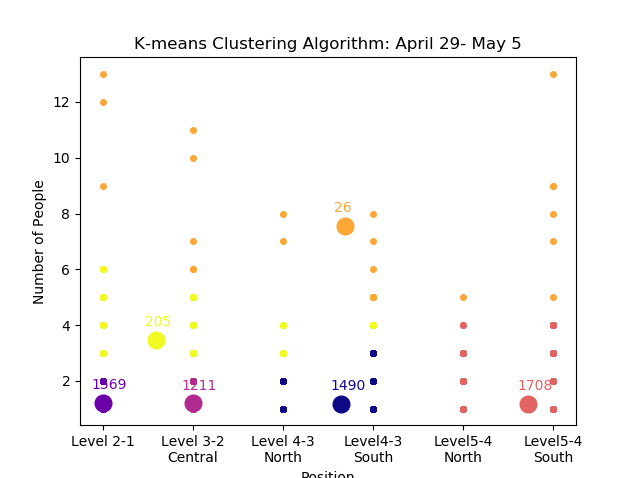
\includegraphics[width=.5\textwidth]{image/Chapters/Chapter6/kmeans1WeekDuring.png}%29apriloneweek
    \caption{K-means algorithm is applied on e-counter data for one week(first week of intervention 29april- 5 may).}
    \label{elbkmean}
\end{figure}    






\begin{figure}[]
    \centering
    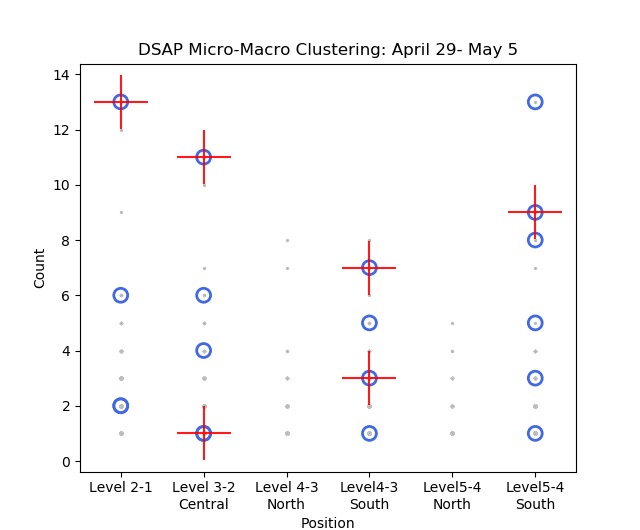
\includegraphics[width=.49\textwidth]{image/Chapters/Chapter6/during3hour-samp 9.preference 1.No Thre.png}
    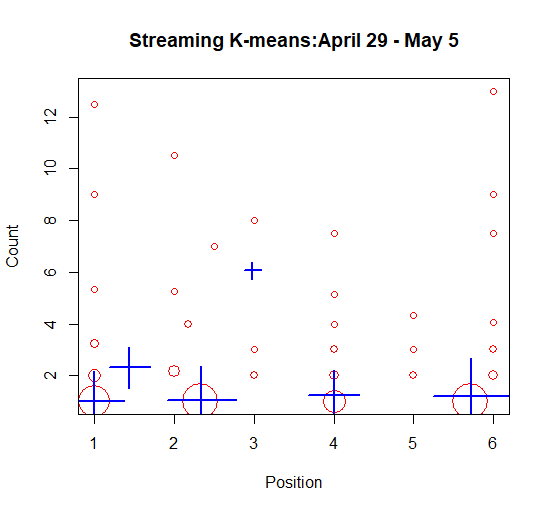
\includegraphics[width=.49\textwidth]{image/Chapters/Chapter6/StreamKDuring.png}
    \caption{Clustering results from DSAP and streaming K-means algorithms applied on the e-counter data for the first week of intervention 29 April- 5 May. window size =5 hour, damping = 0.9, expiration value = 50.}
    \label{6}
\end{figure}



\begin{figure}[!h]
    \centering
   
    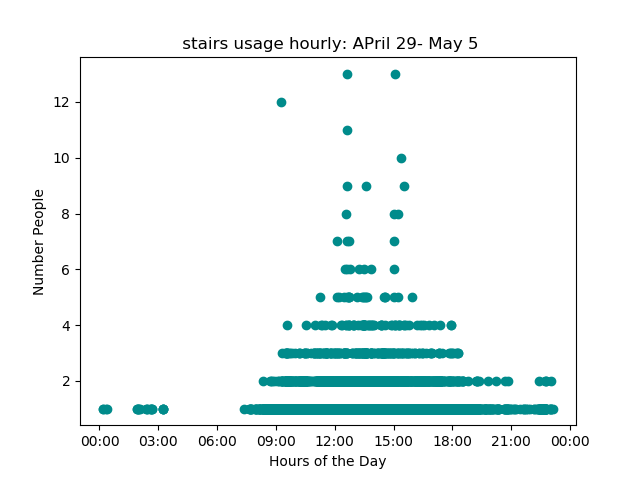
\includegraphics[width=0.5\textwidth]{image/Chapters/Chapter6/oneWeekhourly.png}\hfill
    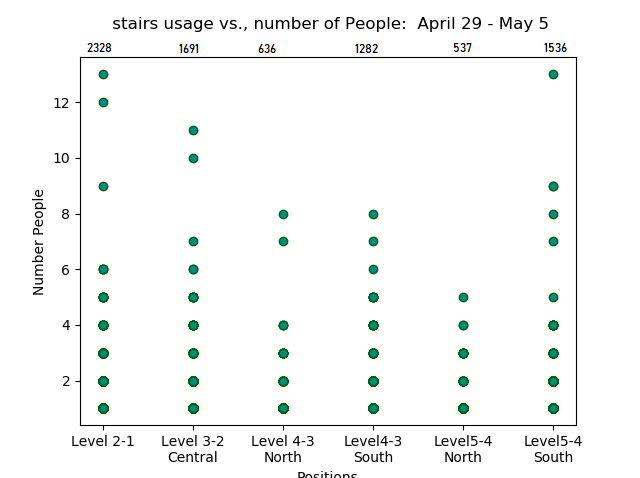
\includegraphics[width=0.5\textwidth]{image/Chapters/Chapter6/PositionCountOneWeek.png}\hfill
    \includegraphics[width=0.5\textwidth]{image/Chapters/Chapter6/oneweekCountDistributon.png}\hfill 
    \includegraphics[width=0.5\textwidth]{image/Chapters/Chapter6/oneweekPositionDistributon.png}
    \caption{One week data distribution. First week of intervention from April 29 -May 5.}
    \label{5}
\end{figure}



\begin{table}[!h]
\small
\caption{Comparison of AP, DSAP, K-means, and Streaming K-means Evaluation Metrics for the first week of intervention (Apr 29 - May 5).AP: Damping=0.96 and preference is the median value of the similarity matrix.}
\label{all3}
\begin{tabular}{l
>{\columncolor[HTML]{CBCEFB}}c 
>{\columncolor[HTML]{FFCCC9}}c 
>{\columncolor[HTML]{CBCEFB}}c 
>{\columncolor[HTML]{FFCCC9}}c }
\hline
\multicolumn{1}{c}{\textbf{Metrics}} & \textbf{AP} & {\color[HTML]{333333} \textbf{K-means}} & \textbf{DSAP} & \textbf{Streaming K-means} \\ \hline\midrule
\textbf{Processing time (s)}         & 26          & 0.3                                                             & 0.69          & 0.45                       \\ \hline
\textbf{Memory consumption (MB)}     & 519         & 586                                                             & 212           & 213                        \\ \hline
\textbf{Number of clusters}          & 14          & 6                                                               & 11            & 6                          \\ \hline
\textbf{Silhouette Index}      & 0.47        & 0.6                                                             & 0.4           & 0.7                       \\ \hline
\textbf{Caliński-Harabasz Index}     & 1421        & 12341                                                            & 35            & 100                         \\ \hline
\textbf{Davies-Bouldin Index}        & 0.57        & 0.68                                                            & 0.49          & 0.31                        \\ \hline\midrule
\end{tabular}
\end{table}





%%%%%%%%%%%%%%%%%%%%%%%%%%%%%%%%%%%%%%%%%%%%%%%%%%%%%%%%%%%%%%%%%%%%%%  After Intervention
\begin{figure}[!h]
    \centering
    \includegraphics[width = 11 cm]{image/Chapters/Chapter6/ApFirstWeekAfterInt.png}
    \caption{AP algorithm is applied on e-counter data for one week. The first week after intervention. with the damping = 0.96 and preference(np.median(similarity matrix)=.7  }
    \label{apaft}
\end{figure}




\begin{figure}[!h]
    \centering
    \includegraphics[width=.49\textwidth]{image/Chapters/Chapter6/elbowAfterInt.png}
    \includegraphics[width=.49\textwidth]{image/Chapters/Chapter6/kmeans1WeekAfter.png}
    \caption{K-means algorithm is applied on e-counter data for one week(first week after intervention: May 27- June 2).}
    \label{elbkmean}
\end{figure}   







\begin{figure}[]
    \centering
    \includegraphics[width=.49\textwidth]{image/Chapters/Chapter6/After5hour-samp 9.preference 4.No Thre.png}
    \includegraphics[width=.49\textwidth]{image/Chapters/Chapter6/StreamKAfter.png}
    \caption{Clustering results from DSAP and streaming K-means algorithms applied on the e-counter data for the first week after intervention. window size =5 hour, damping = 0.9, expiration value = 50.}
    \label{36}
\end{figure}



\begin{figure}[!h]
    \centering
      \includegraphics[width=0.5\textwidth]{image/Chapters/Chapter6/oneWeekAfterhourly.png}\hfill
    \includegraphics[width=0.5\textwidth]{image/Chapters/Chapter6/PositionCountOneWeekAfter.png}\hfill
    \includegraphics[width=0.5\textwidth]{image/Chapters/Chapter6/oneweekCountDistributonAfter.png}\hfill 
    \includegraphics[width=0.5\textwidth]{image/Chapters/Chapter6/oneweekafterPositionDistributon.png}
    \caption{One week data distribution. First week after intervention from May 27- June 2.}
    \label{55}
\end{figure}





\begin{table}[!h]
\small
\caption{Comparison of AP, DSAP, K-means, and Streaming K-means Evaluation Metrics for the first week after intervention (May 27- June 2 ).}
\label{Aftcom}
\begin{tabular}{l
>{\columncolor[HTML]{CBCEFB}}c 
>{\columncolor[HTML]{FFCCC9}}c 
>{\columncolor[HTML]{CBCEFB}}c 
>{\columncolor[HTML]{FFCCC9}}c }
\hline
\multicolumn{1}{c}{\textbf{Metrics}} & \textbf{AP} & {\color[HTML]{333333} \textbf{K-means}} & \textbf{DSAP} & \textbf{Streaming K-means} \\ \hline\midrule
\textbf{Processing time (s)}         & 20          & 0.33                                    & 0.71          & 0.67                       \\ \hline
\textbf{Memory consumption (MB)}     & 541         & 570                                     & 212           & 214                        \\ \hline
\textbf{Number of clusters}          & 19          & 6                                       & 10            & 6                          \\ \hline
\textbf{Silhouette Index}      & 0.14        & 0.6                                     & 0.4           & 0.6                        \\ \hline
\textbf{Caliński-Harabasz Index}     & 278         & 11574                                   & 50            & 80                         \\ \hline
\textbf{Davies-Bouldin Index}        & 0.64        & 0.6                                     & 0.66          & 0.42                       \\ \hline\midrule
\end{tabular}
\end{table}





% \begin{figure}[!h]
%     \centering
%     \includegraphics[width = 11 cm]{image/Chapters/Chapter6/firstweekinterK.png}%firstweekinter
%     \caption{Streaming K-means algorithm is applied on e-counter data for one week.first week of intervention: 29 April- 5 May.}
%     \label{oneweekKmean}
% \end{figure}

%%%%%%%% Comparison table






% \begin{table}[ht]
%     \centering
%     \caption{AP Evaluation Metrics for first week of intervention}
%     \label{dsap12}
%     \begin{tabular}{|c|c|}
%     \hline
%       Metrics & Values  \\
%      \hline
%       Processing time (s)   & 101        \\
%      \hline
%       Memory consumption (MB)   &  612    \\
%      \hline
%       Number of clusters  &  15     \\
%       \hline
%       Silhouette Coefficient    &    0.33 \\
%     \hline
%     Calinski-Harabasz Index     & 1563       \\
%     \hline
%      Davies-Bouldin Index   &     0.59  \\
%     \hline
%     \end{tabular}
% \end{table}


% \begin{table}[ht]
%     \centering
%     \caption{K-means Evaluation Metrics for first week of intervention}
%     \label{dsap12}
%     \begin{tabular}{|c|c|}
%     \hline
%       Metrics & Values  \\
%      \hline
%       Processing time (s)   & 3        \\
%      \hline
%       Memory consumption (MB)   &  222    \\
%      \hline
%       Number of clusters  &  4     \\
%       \hline
%       Silhouette     &    0.63 \\
%     \hline
%     Calinski-Harabasz Index     & 1303       \\
%     \hline
%      Davies-Bouldin Index   &     0.68  \\
%     \hline
%     \end{tabular}
% \end{table}


% \begin{table}[ht]
%     \centering
%     \caption{DSAP Evaluation Metrics for first week of intervention}
%     \label{dsap12}
%     \begin{tabular}{|c|c|}
%     \hline
%       Metrics & Values  \\
%      \hline
%       Processing time (s)   & 19        \\
%      \hline
%       Memory consumption (MB)   &  270    \\
%      \hline
%       Number of macro clusters  &  7     \\
%       \hline
%       Silhouette Coefficient    &    0.87 \\
%     \hline
%     Calinski-Harabasz Index     & 20891       \\
%     \hline
%      Davies-Bouldin Index   &     0.52  \\
%     \hline
%     \end{tabular}
% \end{table}


The memory and time advantages offered by the DSAP algorithm is obvious from the comparisons shown with the data from the first week of intervention. The people counter experiment was performed in order to find any improvement in stair usage after some measures for educational interference were taken. In order to analyze this the DSAP algorithm was applied on each of the months before, during, and after intervention using a landmark time window of 4 hours. The resulting clusters are shown in Figure \ref{dsap3mon}. It shows ..xx
For comparison, the clusters obtained by the streaming k-means method are plotted in Figure. xx

Comparison table and closing inference..xx
\begin{figure}[!h]
    \centering
    \includegraphics[width=.47\textwidth]{image/Chapters/Chapter6/DSAPBeforeMonthIntervention.png}
    \includegraphics[width=.51\textwidth]{image/Chapters/Chapter6/window10H.png}
    \includegraphics[width=.49\textwidth]{image/Chapters/Chapter6/DSAPAFTERmonthIntervention.png}
    \caption{The clusters obtained by the DSAP algorithm from the e-counter data for one month periods before, during, and after intervention.}
    \label{dsap3mon}
\end{figure}

% \begin{figure}
%     \centering
%     \includegraphics[width = 11 cm]{image/Chapters/Chapter6/DSAPBeforeMonthIntervention.png}%ecounter_time data
%     \caption{DSAP algorithm is applied on e-counter data for one month before intervention.}
%     \label{}
% \end{figure}


% \begin{figure}
%     \centering
%     \includegraphics[width = 11 cm]{image/Chapters/Chapter6/window10H.png}%ecounter_time data
%     \caption{DSAP algorithm is applied on e-counter data for one month of intervention.}
%     \label{}
% \end{figure}



% \begin{figure}
%     \centering
%     \includegraphics[width = 11 cm]{image/Chapters/Chapter6/DSAPAFTERmonthIntervention.png}%ecounter_time data
%     \caption{DSAP algorithm is applied on e-counter data for one month after intervention.}
%     \label{}
% \end{figure}



% \begin{table}[ht]
%     \centering
%     \caption{DSAP Evaluation Metrics }
%     \label{dsap12}
%     \begin{tabular}{|c|c|c|c|}
%     \hline
%       Metrics & Before Intervention &  Intervention & After Intervention  \\
%      \hline
%       Processing time (s)   & 19.05          &   19.3 &  18.8 \\
%      \hline
%       Memory consumption (MB)   &  208     & 220     & 240\\
%      \hline
%       Number of micro clusters  &  29      & 43     & 64\\
%       \hline
%       Number of macro clusters  &   7     &  7     & 8 \\
%      \hline
%       Silhouette Coefficient    &    0.33  & 0.62    & 0.57\\
%     \hline
%     Calinski-Harabasz Index     & 64      & 216      &  89  \\
%     \hline
%      Davies-Bouldin Index   &     0.69   & 0.44        &    0.48\\
%     \hline
%     \end{tabular}
% \end{table}

% \begin{figure}[!h]
%     \centering
%     \includegraphics[width=.5\textwidth]{image/Chapters/Chapter6/elbow_onemonth.png}%29apriloneweek data
%     \includegraphics[width=.5\textwidth]{image/Chapters/Chapter6/kmeans_onemonth.png}%29apriloneweek
%     \caption{K-means algorithm is applied on e-counter data for one month(intervention month).}
%     \label{kstream}
% \end{figure} 


%%%%%%%%%%%%%%%% data analysis
%%%%%%%%% one moth DSAP for 3 month
%%%%%%%% one m SKM



% \begin{table}[ht]
%     \centering
%     \caption{DSAP Evaluation Metrics for first week of intervention}
%     \label{dsap12}
%     \begin{tabular}{|c|c|}
%     \hline
%       Metrics & Values  \\
%      \hline
%       Processing time (s)   & 101        \\
%      \hline
%       Memory consumption (MB)   &  612    \\
%      \hline
%       Number of micro clusters  &  15     \\
%       \hline
%       Number of macro clusters  &   7     \\
%      \hline
%       Silhouette Coefficient    &    0.33 \\
%     \hline
%     Calinski-Harabasz Index     & 64       \\
%     \hline
%      Davies-Bouldin Index   &     0.69  \\
%     \hline
%     \end{tabular}
% \end{table}


%DSAP2
% \begin{figure}
%     \includegraphics[width=.5\textwidth]{image/before-1 month3.png}\hfill
%     \includegraphics[width=.5\textwidth]{image/during-1 month3.png}\hfill\centering
%     \includegraphics[width=.5\textwidth]{image/after-1 month3.png}
%     \\[\smallskipamount]
%     \caption{DSAP v.1 results. Dataset: people counter; monthly}
%     \label{ds1}
% \end{figure}


% \begin{figure}
%     \includegraphics[width=.5\textwidth]{image/3.18.png}\hfill
%     \includegraphics[width=.5\textwidth]{image/F5.2igure_1.png}\hfill\centering
%     \includegraphics[width=.5\textwidth]{image/6.10.png}
%     \\[\smallskipamount]
%     \caption{DSAP v.2 results. Dataset: people counter, one week of before, during and after intervention}
%     \label{dspp2}
% \end{figure}




% \subsection{ Performance Evaluation of the AP, DSAP, K-means and Streaming K-means Clustering Algorithms}

% The performance and scaling of clustering algorithms can be related to the implementation of the underlying algorithm. A well-written implementation and data structures used have a large impact on an increase in the performance of algorithms.     
% To begin with, we need to get together all the clustering implementations, by plotting libraries to see what is going on once data is plotted. The implementations tested with AP, K-means, DSAP and Streaming K-means. Except the Streaming K-means which is implemented in RStudio, others are implemented in Python.

% A major factor in performance is algorithm itself. For example, AP. AP needs to calculate four matrices which makes it slow.
% then benchmarking code at various dataset sizes are tested. Because algorithms may have different performance depending on the dataset. Also, these algorithms are run several times on datasets to get the average performance.

% \subsection{Evaluation Criterion}
% Evaluating the quality of clustering algorithms
% Cluster analysis itself is not an algorithm. It can be obtained by different algorithms that differ significantly in their understanding of what constitutes a cluster. Common criteria of clusters include groups with short distances between cluster members, dense areas of the data points, intervals or particular statistical distributions.

% The empirical study chooses four clustering algorithms, three validity measures to validate the evaluation approach.




\begin{figure}[!h]
    \centering
    \includegraphics[width = 7.5 cm]{image/Chapters/Chapter6/time.point.lessinitial.png}\hfill
    \includegraphics[width = 7.5 cm]{image/Chapters/Chapter6/mem.point.lessinitial.png}
    \\[\smallskipamount]    
    \caption{ Evaluate DSAP with time and memory per window size which starts from 1000 up to 11000 data points. It was tested on one month e-counter dataset with the expiration time=15.}
    \label{4}
\end{figure}











%%%%%%%%%%%%%%%%%%%%%%%%%%%%%%%%%%%%%%%%%%%%%%%%%%%%%%%%%%%%%%%%%%%%%%%%%%%%%%%%%%%%%%%%%%%%%%%%

\section{Occupant Behaviour Experiment}

This experiment is located at three buildings of at the UJI university campus with three buildings and four to five floors. In this scenario, buildings are named with order from one to three which related to campus building T1, TD and TC which TC is the only building with five floors as shown in Figure \ref{nama} (a) and the 3D plot of all levels and buildings are plotted in Figure \ref{nama} (b), which colors are show different floor in all buildings. 

\begin{figure}[!h]
    \centering
    \includegraphics[width = 7 cm]{image/Chapters/Chapter6/LatLong.png}\hfill
    \includegraphics[width = 8 cm]{image/Chapters/Chapter6/LatLongFloor.png}
    \\[\smallskipamount]    
    \caption{(a) Latitude, Longitude of all data points (people) in three buildings. (b) shows the building floors in 3D view.}
    \label{nama}
\end{figure}


Over the one month of experience, data collected in six days from May 30 until June 20 as depicted in Figure \ref{timeline}. 



\begin{figure}
    \centering
    \includegraphics[width = 12 cm]{image/Chapters/Chapter6/timedist.png}
    \caption{Data Distribution for all days data collected during the experiment duration: May 30 - June 20, 2013. The first 5  days from May 30 until June 12, data collected from building 1 and June 20 is the days data collected from building 2 and 3.}
    \label{timeline}
\end{figure}





The total number of people with their phones participated in this experiment is shown in Figure \ref{userphone}. Phones number 8 and 9 have more activity than other phones. phone number 8 belongs to user number 11, and phone number 9 used by three users with the number 1, 9, and 16.

\begin{figure}[!h]
    \centering
    \includegraphics[width=.5\textwidth]{image/Chapters/Chapter6/userID_data.png}\hfill
    \includegraphics[width=.5\textwidth]{image/Chapters/Chapter6/phoneID_data.png}
    \\[\smallskipamount]    
    \caption{Activity of users and phone during this experiment. user number 11 with the phone number 8 and users number 1,9, and 16 with the same phone number 9 have the most movement in the building.}
    \label{userphone}
\end{figure}


Moreover, Figure \ref{phoneall} illustrated the phones spread in these three building during the experiment. As it is shown, the only phones were in the building T1 (first building) was phones number8 and 9. 


\begin{figure}
    \centering
    \includegraphics[width = 10 cm]{image/Chapters/Chapter6/LatLongUser.png}
    \caption{Real-world position of each phone in buildings T1(First one on the left), TD (middle building), and TC(right side of the figure).}
    \label{phoneall}
\end{figure}





As shown in Figure \ref{bdd}, the TC has significantly more number of data point in compare with other building  and it means people usually was in the third building. Also, pie chart in Figure \ref{Pfloor} shows that almost all buildings floor are equally occupied by user and the exception is level five, as mentioned before, it just belongs to TC building. Moreover, as depicted in Figure \ref{spaceiduniq }, all rooms, classes, lab, offices etc., has a number referrers from 0 to 732 for  buildings T1, TD, and TC Respectively. Space ID from 0 to 255 belongs to building T1, numbers between 256 to 416 belong to building TD, and the rest of it (417 to 732) includes space in building TC.



\begin{figure}
    \centering
    \includegraphics[width = 12 cm]{image/Chapters/Chapter6/buidlingID.png}
    \caption{Buildings data distribution during experiment. }
    \label{bdd}
\end{figure}




%%%% NEMODAR ZAman tanha


\begin{figure}
    \centering
    \includegraphics[width = 12 cm]{image/Chapters/Chapter6/floors.png}
    \caption{Pie chart of activities in all Floors in three building during the experiment }
    \label{Pfloor}
\end{figure}





\begin{figure}
    \centering
    \includegraphics[width = 16 cm]{image/Chapters/Chapter6/uniqspaceid.png}
    \caption{Histogram of spaceid distribution during the entire experiment. Each color related to one building.Numbers from 0-255 are in building 1, 256- 416 are in building 2 and 417-732 are located in building 3.}
    \label{spaceiduniq }
\end{figure}






Figures \ref{alltogether} illustrate the movement of people during the experiment period. 







\begin{figure}
    \centering
        \includegraphics[width = 7 cm]{image/Chapters/Chapter6/phoneTime.png}\hfill
        \includegraphics[width = 7 cm]{image/Chapters/Chapter6/spaceidAccumulat.png}\hfill
        \includegraphics[width = 7 cm]{image/Chapters/Chapter6/floorTime.png}\hfill
        \includegraphics[width = 7 cm]{image/Chapters/Chapter6/buildingTime.png}
    \caption{(a) Phone activity level during the entire experiment time. (b) Space activity level during the entire experiment time. (c) Floor activity during the entire experiment time. (d) Building activity level during the entire experiment time.}
    \label{alltogether}
\end{figure}




% \begin{figure}
%     \centering
%     \includegraphics[width = 15 cm]{image/Chapters/Chapter6/phoneTime.png}
%     \caption{Phone activity level during the entire experiment time. }
%     \label{phonetime}
% \end{figure}


% \begin{figure}
%     \centering
%     \includegraphics[width = 15 cm]{image/Chapters/Chapter6/buildingTime.png}
%     \caption{Building activity level during the entire experiment time. }
%     \label{buildtime}
% \end{figure}



% \begin{figure}
%     \centering
%     \includegraphics[width = 15 cm]{image/Chapters/Chapter6/floorTime.png}
%     \caption{Floor activity during the entire experiment time. }
%     \label{floract}
% \end{figure}





% \subsection{Comparison of Data clustering Algorithms}

The UJIIndoorLoc dataset is similarly happened as the e-counter dataset. To find a pattern in this data, first AP and K-means clustering algorithms were performed to find people activities in these three buildings during experiment period. As our computer used for this study could not handle the whole experience duration for clustering data by AP, the 20 of June is selected for our experiment . This day includes almost all people in the experiment but building T1 is not presented in this specific day. The statistic of this day shows in Figure \ref{static} The K-means algorithm was able to handle to total amount of data points.
The streaming affinity propagation algorithm  DSAP was preferred for this study. But, for the sake of completeness and validation, the results from DSAP are compared with those from AP, k-means, and streaming K-means.


\begin{figure}
    \centering
        \includegraphics[width = 7 cm]{image/Chapters/Chapter6/phoneTimejune20png.png}\hfill
        \includegraphics[width = 8 cm, height =160]{image/Chapters/Chapter6/spaceidAccumulatjune20.png}\hfill
        \includegraphics[width = 7 cm]{image/Chapters/Chapter6/floorTimejune20.png}\hfill
        \includegraphics[width = 7 cm]{image/Chapters/Chapter6/buildingTimejun6.png}
    \caption{Activities during one day : June 20, 2013 (a) Phone activity level. (b) Space activity level. (c) Floor activity. (d) Building activity level.}
    \label{static}
\end{figure}





\begin{figure}[!h]
    \centering
    \includegraphics[width = 10 cm]{image/Chapters/Chapter6/APJune20.png}
    \caption{ AP for WiFi data during the experiment: June 20.}
    \label{APUjoneday}
\end{figure}


Figure \ref{APUjoneday} shows the clusters generated by the AP algorithm for June 20, 2013. AP clustering algorithm, divided the data in to five clusters.


Figure \ref{elbowkwifi} shows the elbow method to find the optimal number of clusters for K-means algorithm and seems to be six for this day. The corresponding clusters using k-means are shown in the right of this figure. %Explain clusters


\begin{figure}[!h]
    \centering
    \includegraphics[width = 7.5 cm]{image/Chapters/Chapter6/elbowDay20.png}\hfill
     \includegraphics[width = 7.5 cm]{image/Chapters/Chapter6/kmeansJun20.png}
    \\[\smallskipamount]    
    \caption{Kmeans for WiFi data : June 20.}
    \label{elbowkwifi}
\end{figure}







\begin{figure}[!h]
    \centering
    \includegraphics[width = 7 cm]{image/Chapters/Chapter6/DSAPJune20.png}\hfill
    \includegraphics[width = 7 cm]{image/Chapters/Chapter6/june20DoubK.png}
    \\[\smallskipamount]    
    \caption{ DSAP and Streaming K-means for WiFi data during the experiment: June 20.}
    \label{3}
\end{figure}


% Please add the following required packages to your document preamble:
% \usepackage[table,xcdraw]{xcolor}
% If you use beamer only pass "xcolor=table" option, i.e. \documentclass[xcolor=table]{beamer}
\begin{table}[]
\small
\caption{Comparison of AP, DSAP, K-means, and Streaming K-means Evaluation Metrics for the day June 6.}
\label{Wificom}
\begin{tabular}{l
>{\columncolor[HTML]{DAE8FC}}c 
>{\columncolor[HTML]{68CBD0}}c 
>{\columncolor[HTML]{DAE8FC}}c 
>{\columncolor[HTML]{68CBD0}}c }
\hline
\multicolumn{1}{c}{\textbf{Metrics}} & \textbf{AP} & {\color[HTML]{333333} \textbf{K-means}} & \textbf{DSAP} & \textbf{Streaming K-means} \\ \hline\midrule
\textbf{Processing time (s)}         & 414         & 1.9                                     & 2.2             & 0.58                       \\ \hline
\textbf{Memory consumption (MB)}     & 1933        & 412                                     & 290           & 238                        \\ \hline
\textbf{Number of clusters}          & 5           & 6                                       & 6             & 6                          \\ \hline
\textbf{Silhouette Index}      & 0.3         & 0.5                                     & 0.55          &                            \\ \hline
\textbf{Caliński-Harabasz Index}     & 7193        & 25330                                   & 365           &                            \\ \hline
\textbf{Davies-Bouldin Index}        & 0.7         & 0.6                                     & 0.57          &                            \\ \hline\midrule
\end{tabular}
\end{table}





\begin{figure}[!h]
    \centering
    \includegraphics[width = 7.5 cm]{image/Chapters/Chapter6/elbowWholeWifiNormalize.png}\hfill
     \includegraphics[width = 7.5 cm]{image/Chapters/Chapter6/kmeanswifiAllDays.png}
    \\[\smallskipamount]    
    \caption{Kmeans for WiFi data during the experiment: May 30 - June 20.}
    \label{2}
\end{figure}






\begin{figure}[!h]
    \centering
    \includegraphics[width = 10 cm]{image/Chapters/Chapter6/DSAPalldays.png}
    \caption{ DSAP for WiFi data during the experiment: May 30 - June 20.}
    \label{1}
\end{figure}


 


% \begin{table}[h]
%     \centering
%     \caption{Comparison of AP, DSAP, and K-means Evaluation Metrics for one day of WiFi data (June 20).}
%     \label{comp2}
%     \begin{tabular}{|c|c|c|c|}
%     \hline
%       Metrics & AP & DSAP & K-means  \\
%      \hline
%       Processing time (s)         &   414     &      60      &       1.9     \\
%      \hline
%       Memory consumption (MB)     &   1933    &      202     &      412\\
%      \hline
%       Number of clusters          &   5       &     6        &        6  \\
%       \hline
%       Silhouette Coefficient      &   0.3     &      0.5     &      0.5 \\
%     \hline
%     Calinski-Harabasz Index       &      7193 &       84     &       25330     \\
%     \hline
%      Davies-Bouldin Index         &     0.7   &      0.6     &       0.6\\
%     \hline
%     \end{tabular}
% \end{table}
































% \end{document}